%%%%%%%%%
\section{W+jets background estimate with $\alpha$ ratio method}\label{sec:alpha}
%%%%%%%%%

The $\mlvj$ distribution observed in data is dominated by SM background processes where single
quark or gluon jets are falsely identified as signal jets. The dominant processes is inclusive W boson production. 
Since both normalization and shape discrepancies are visibile between data and simulation~\cite{Chatrchyan:2013vbb},
a data driven method has been developed to estimate this background component, as described in the following.
Sub-dominant backgrounds include \ttbar, single top quark, and non resonant diboson SM production,
which are estimated from MC, after applying correction factors for residual data-to-simulation disagreement measured in control samples selected in data.

\subsection{Background estimation procedure}

The W+jets background is estimated through the so called \textit{$\alpha$ ratio} method.
This method assumes that the correlation between \mJ and $\mlvj$ for the dominant W+jets background can be adequately modelled by simulation.
A signal-depleted control region (sideband) is defined by requiring the mass of the V or H jet to lie below or above the nominal selection; the
$\mlvj$ distribution observed in this region is then extrapolated to the nominal region through
a transfer function estimated from simulation. Other minor sources of background, such as
\ttbar, single top quark, and SM diboson production, are estimated using simulated events after
applying correction factors based on control regions in data, as described in Sections~\ref{sec:vtagging} and~\ref{sec:ttbar}.
The sideband region is defined around the jet mass window that represents the analysis signal region (Section~\ref{sec:finalselection}).
The lower and upper sidebands for the two analyses are summarized in Table~\ref{tab:sidebands}.
For the 13\TeV analysis a ``gap'' is introduced between the signal region and the upper sideband, since the
range defined by $105 < \mJ < 135$ might include contribution from signals with highly Lorentz-boosted Higgs bosons in the final state.
Since these types of searches at 13\TeV~\cite{Khachatryan:2016cfx} have been performed simultaneously with the one described in this work,
this region has been discarded to avoid introducing a bias in the shape and normalization extrapolation due to a possible signal.
On the other hand, the lower sideband of the 8\TeV $\ell\Pgn\bbbar$ analysis includes the region where signals from highly Lorentz-boosted V bosons might occur.
In fact, this analysis has been performed after the search for WV resonances in the semi-leptonic final state at 8\TeV discovered the signal region,
where no deviation from the predicted SM background have been observed~\cite{Khachatryan:2014gha}.

\begin{table}[!htb]
\centering
\caption{Sideband regions used in the two analyses to estimate the contribution from the main W+jets background.}
\begin{tabular}{lcc}
\multirow{2}{*}{{\bf \mJ sideband}} &\multicolumn{2}{c}{{\bf final state}}\\
 & $\ell\Pgn\bbbar$& $\ell\Pgn\qqbar$\\
\hline
\hline
Low sideband (LSB) & 40--110\GeV & 40--65\GeV\\ 
High sideband (HSB) & 135--150\GeV & 135--150\GeV\\ 
\end{tabular}
\label{tab:sidebands}
\end{table}

\subsection{Extraction of the W+jets normalization}

The overall normalization of the W+jets background in the signal region is determined from a
fit to the \mJ distribution in the lower and upper sidebands of the data. The analytical form
of the fitting function is chosen from simulation studies, as are the contributions from minor backgrounds. 
%Figure 3 shows the result of this fit for the low- and high-mass `n+jet channels.
A summary of the empirical functional forms used to parametrize each background contribution are listed in Table~\ref{tab:mjfunct}, and defined as follows:

\footnotesize
\begin{equation}
\begin{gathered}
   F_{\rm Exp}(x)=e^{cx}\\
   F_{\rm ErfExp}(x)=e^{cx} \cdot \frac{1 + {\rm Erf}((x-a)/b)}{2} \\
   F_{\rm ExpGaus}(x) = c_{0} \cdot e^{cx} + c_{1} \cdot \mathrm{Gaus}(x,x_{1},\sigma_{1})\\
   F_{\rm 4Gaus}(x) = c_{1} \cdot \mathrm{Gaus}(x,x_{1},\sigma_{1}) + c_{2} \cdot \mathrm{Gaus}(x,x_{2},\sigma_{2}) + c_{3} \cdot \mathrm{Gaus}(x,x_{3},\sigma_{3}) + c_{4} \cdot \mathrm{Gaus}(x,x_{4},\sigma_{4}) \\
   F_{\rm ErfExp2Gaus}(x) = e^{cx} \cdot \frac{1 + {\rm Erf}((x-a)/b)}{2} + c_{1} \cdot \mathrm{Gaus}(x,x_{1},\sigma_{1}) + c_{2}\cdot \mathrm{Gaus}(x,x_{2},\sigma_{2})\\
\end{gathered}
\label{eqn:mjfunct}
\end{equation}

\normalsize
\begin{table}[!htb]
\centering
\caption{Summary of the empirical functional forms used to fit the \mJ spectra of each background component in the two analyses.}
\begin{tabular}{lcccc}
Final state & W+jets & \ttbar & single top quark & diboson\\
\hline
\hline
$\ell\Pgn\bbbar$ & $F_{\rm ErfExp}(x)$ & $F_{\rm Exp}(x)$ & $F_{\rm Exp}(x)$ & $F_{\rm ExpGaus}(x)$\\
$\ell\Pgn\qqbar$ & $F_{\rm ErfExp}(x)$ & $F_{\rm ErfExp2Gaus}(x)$ & $F_{\rm ExpGaus}(x)$ & $F_{\rm 4Gaus}(x)$
\end{tabular}
\label{tab:mjfunct}
\end{table}

Figure~\ref{fig:mcfits_mj} shows the functional forms listed in Table~\ref{tab:mjfunct} for the $\ell\Pgn\qqbar$ channel, after fitting the simulation data of each background component,
demonstrating that the chosen functions well reproduce the expected \mJ spectra.

\begin{figure}[!htb]
\centering
\subfigure[]{\label{fig:mcfits_mj_a}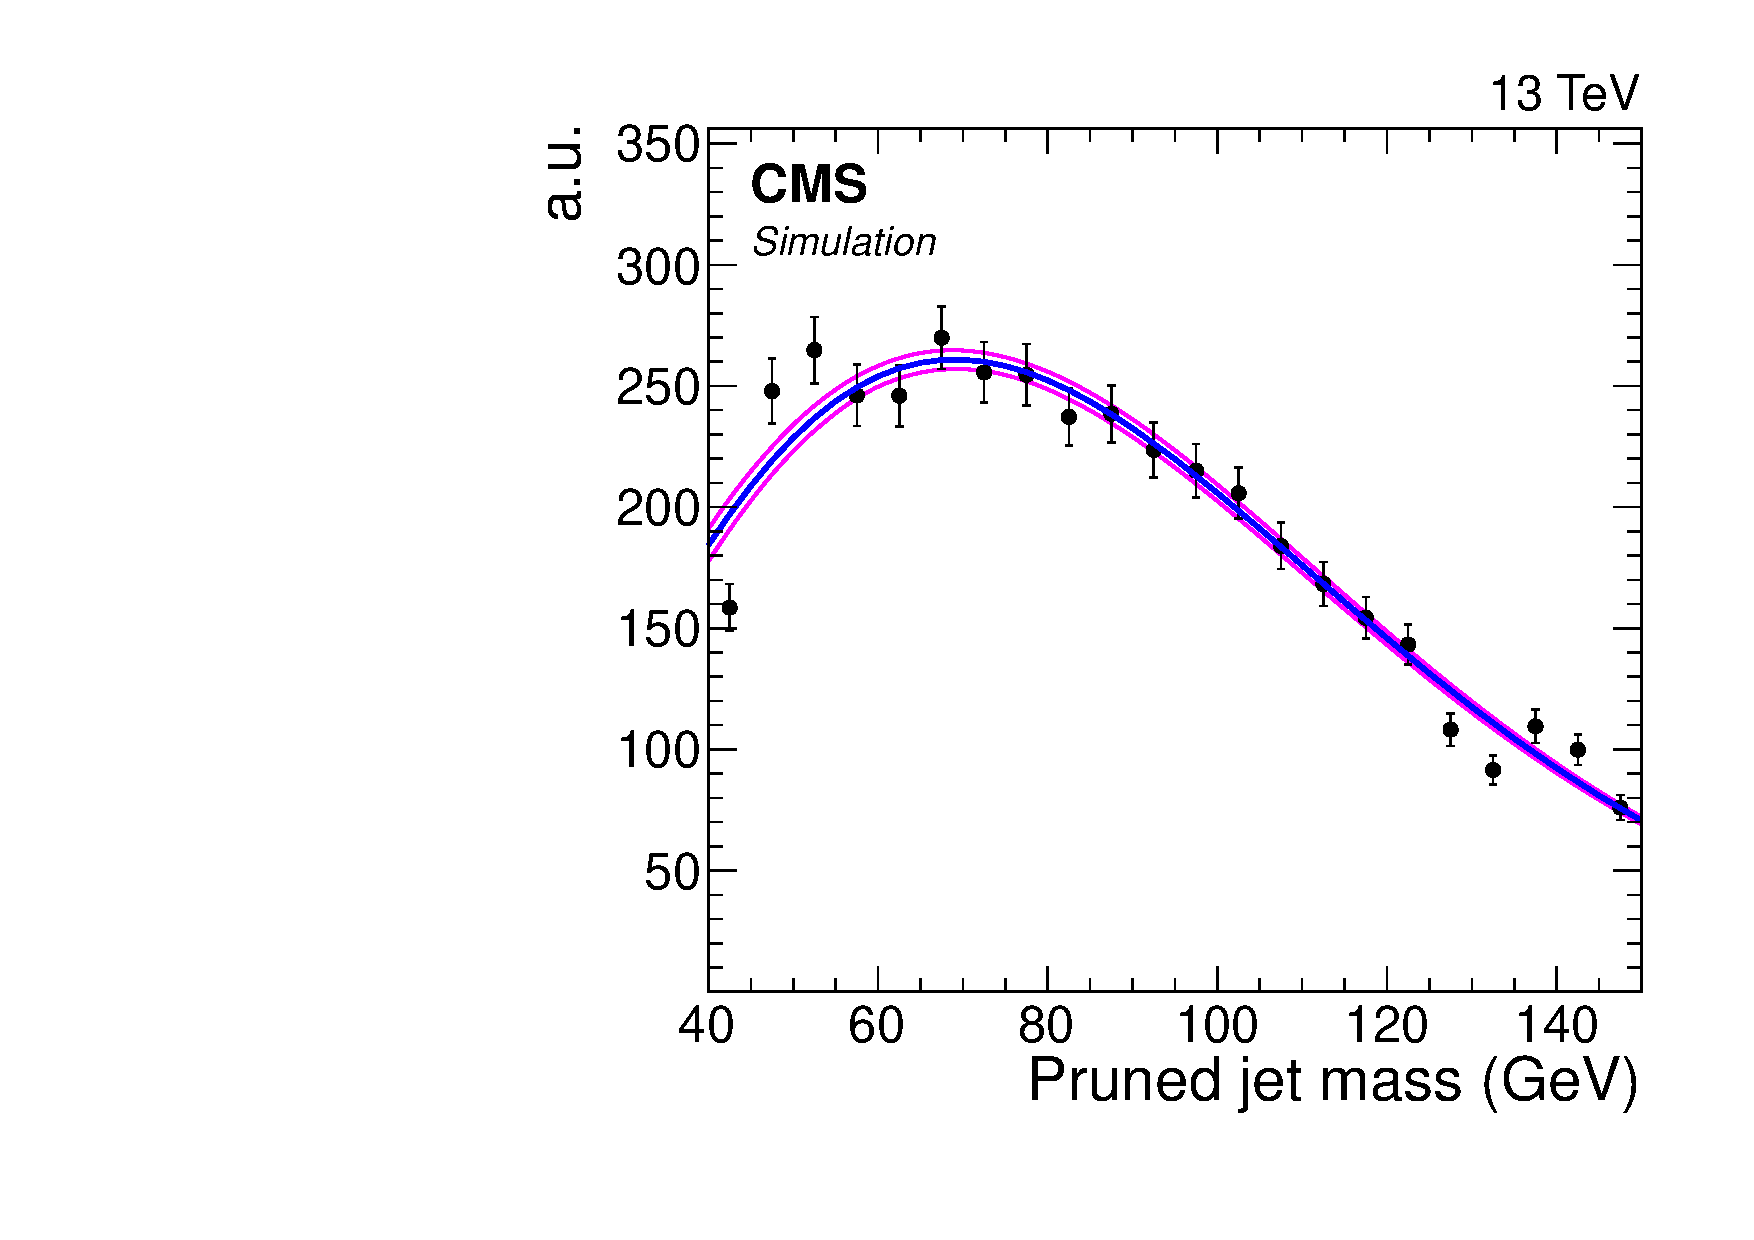
\includegraphics[width=0.45\textwidth]{\cheight/HP_mj_fitting-mu-WJets.pdf}}
\subfigure[]{\label{fig:mcfits_mj_b}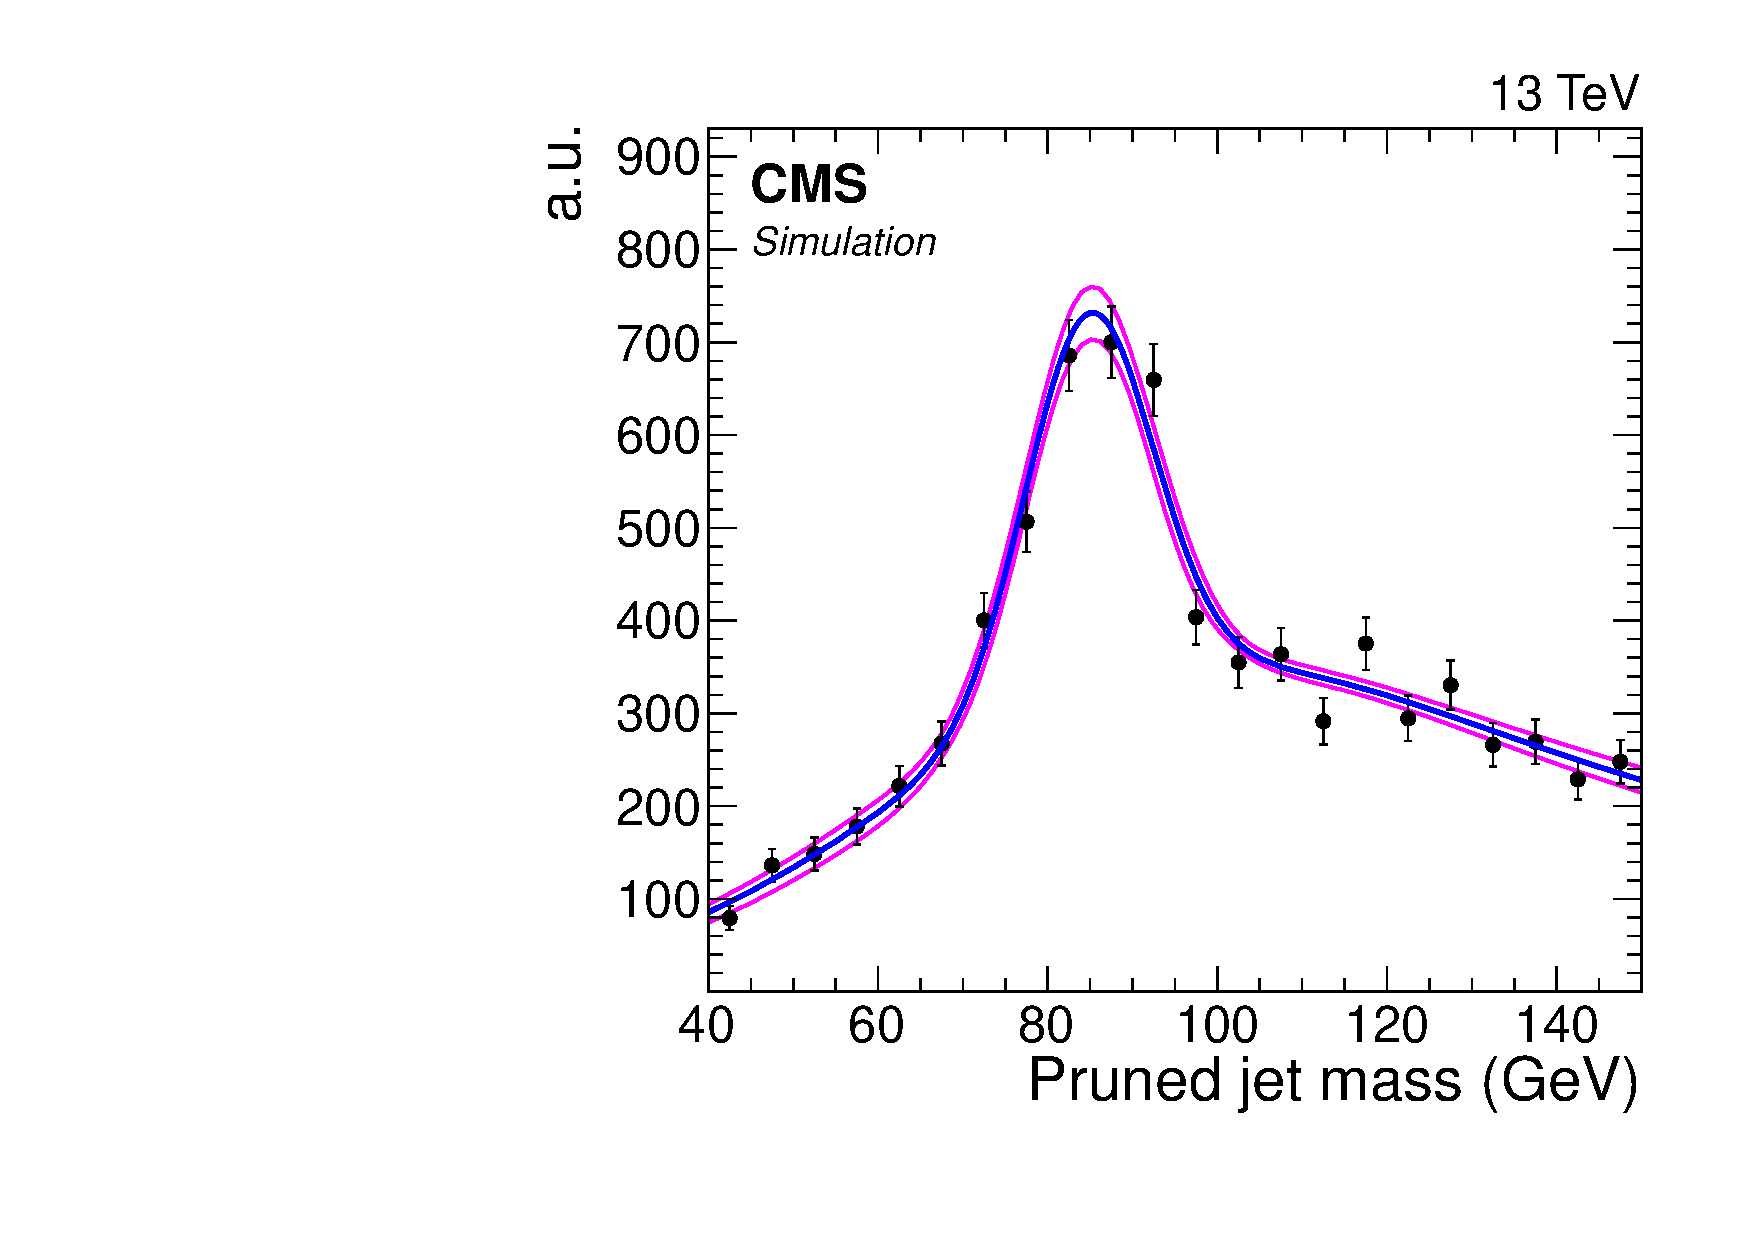
\includegraphics[width=0.45\textwidth]{\cheight/HP_mj_fitting-mu-TTbar.pdf}}\\
\subfigure[]{\label{fig:mcfits_mj_c}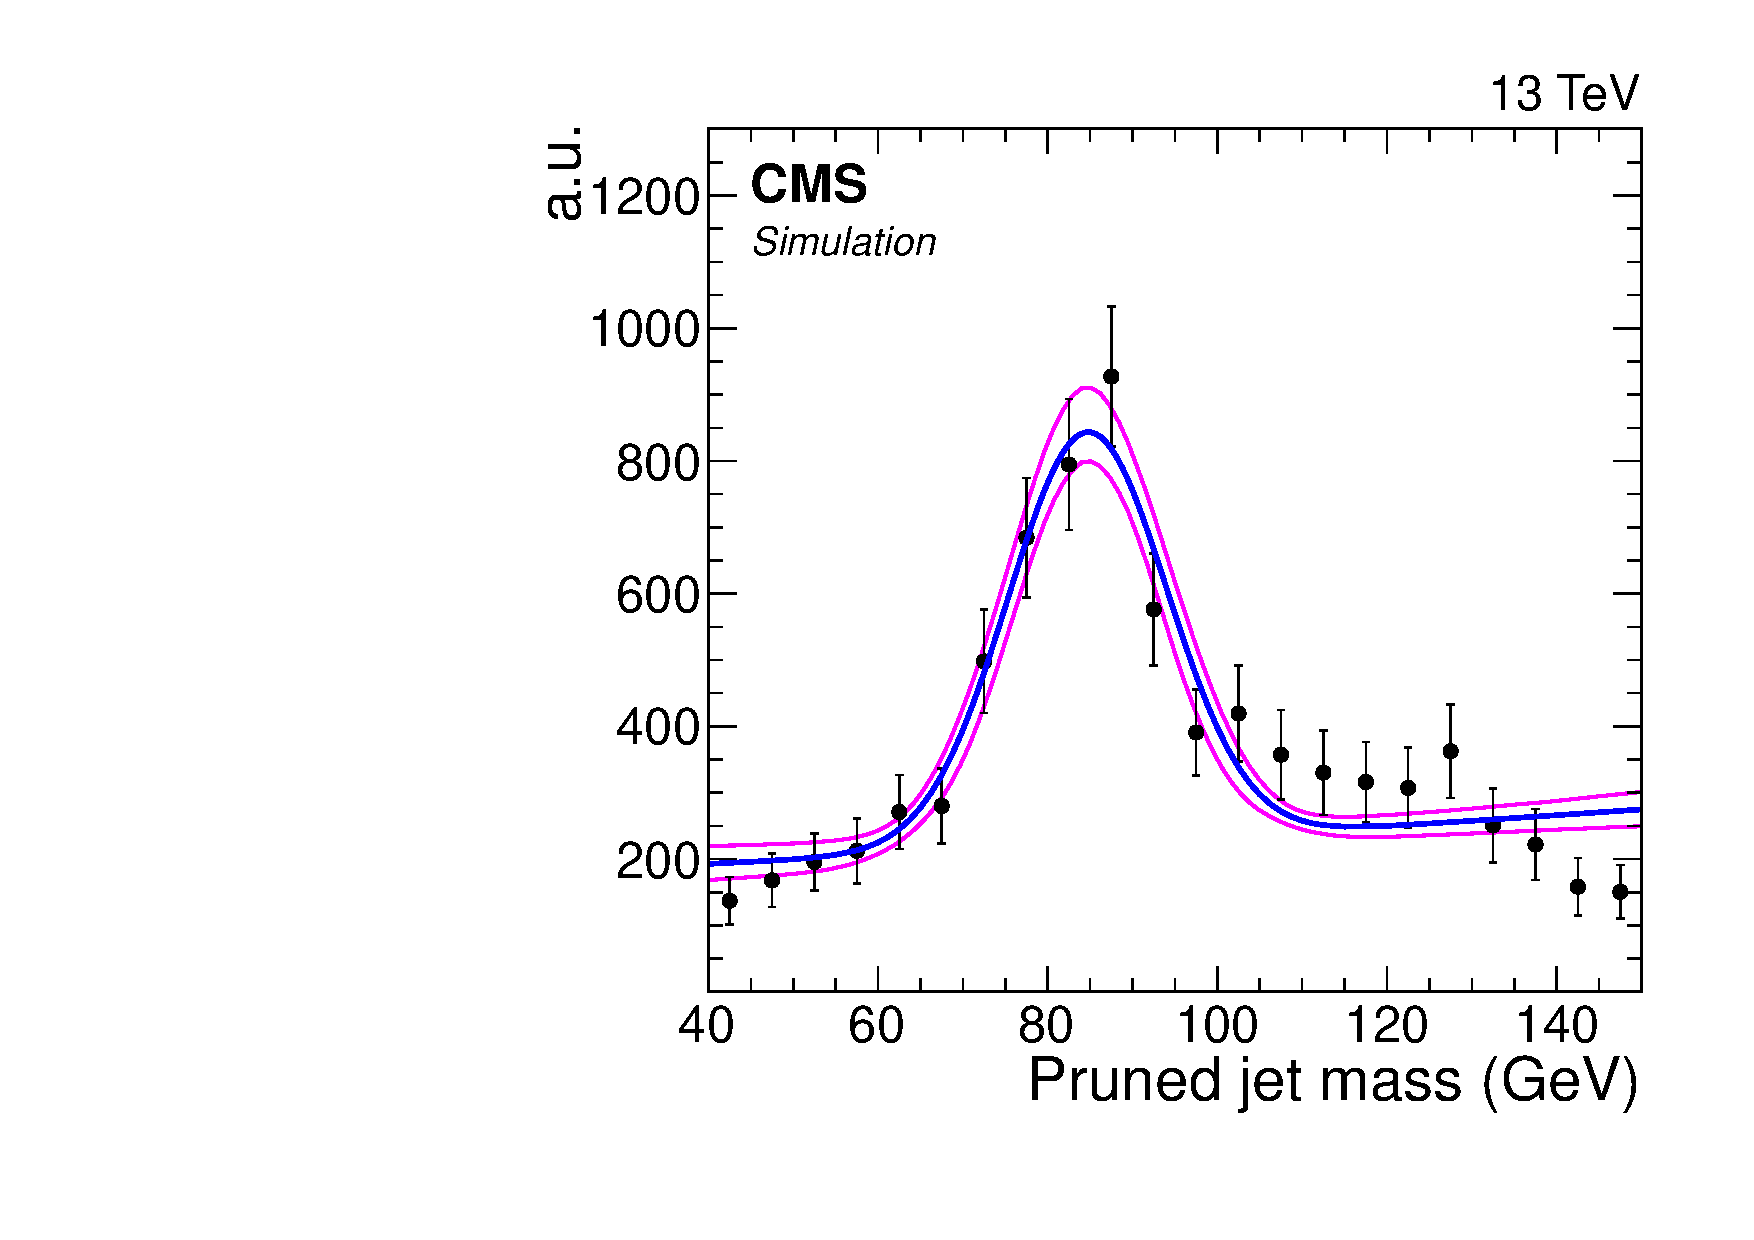
\includegraphics[width=0.45\textwidth]{\cheight/HP_mj_fitting-mu-STop.pdf}}
\subfigure[]{\label{fig:mcfits_mj_d}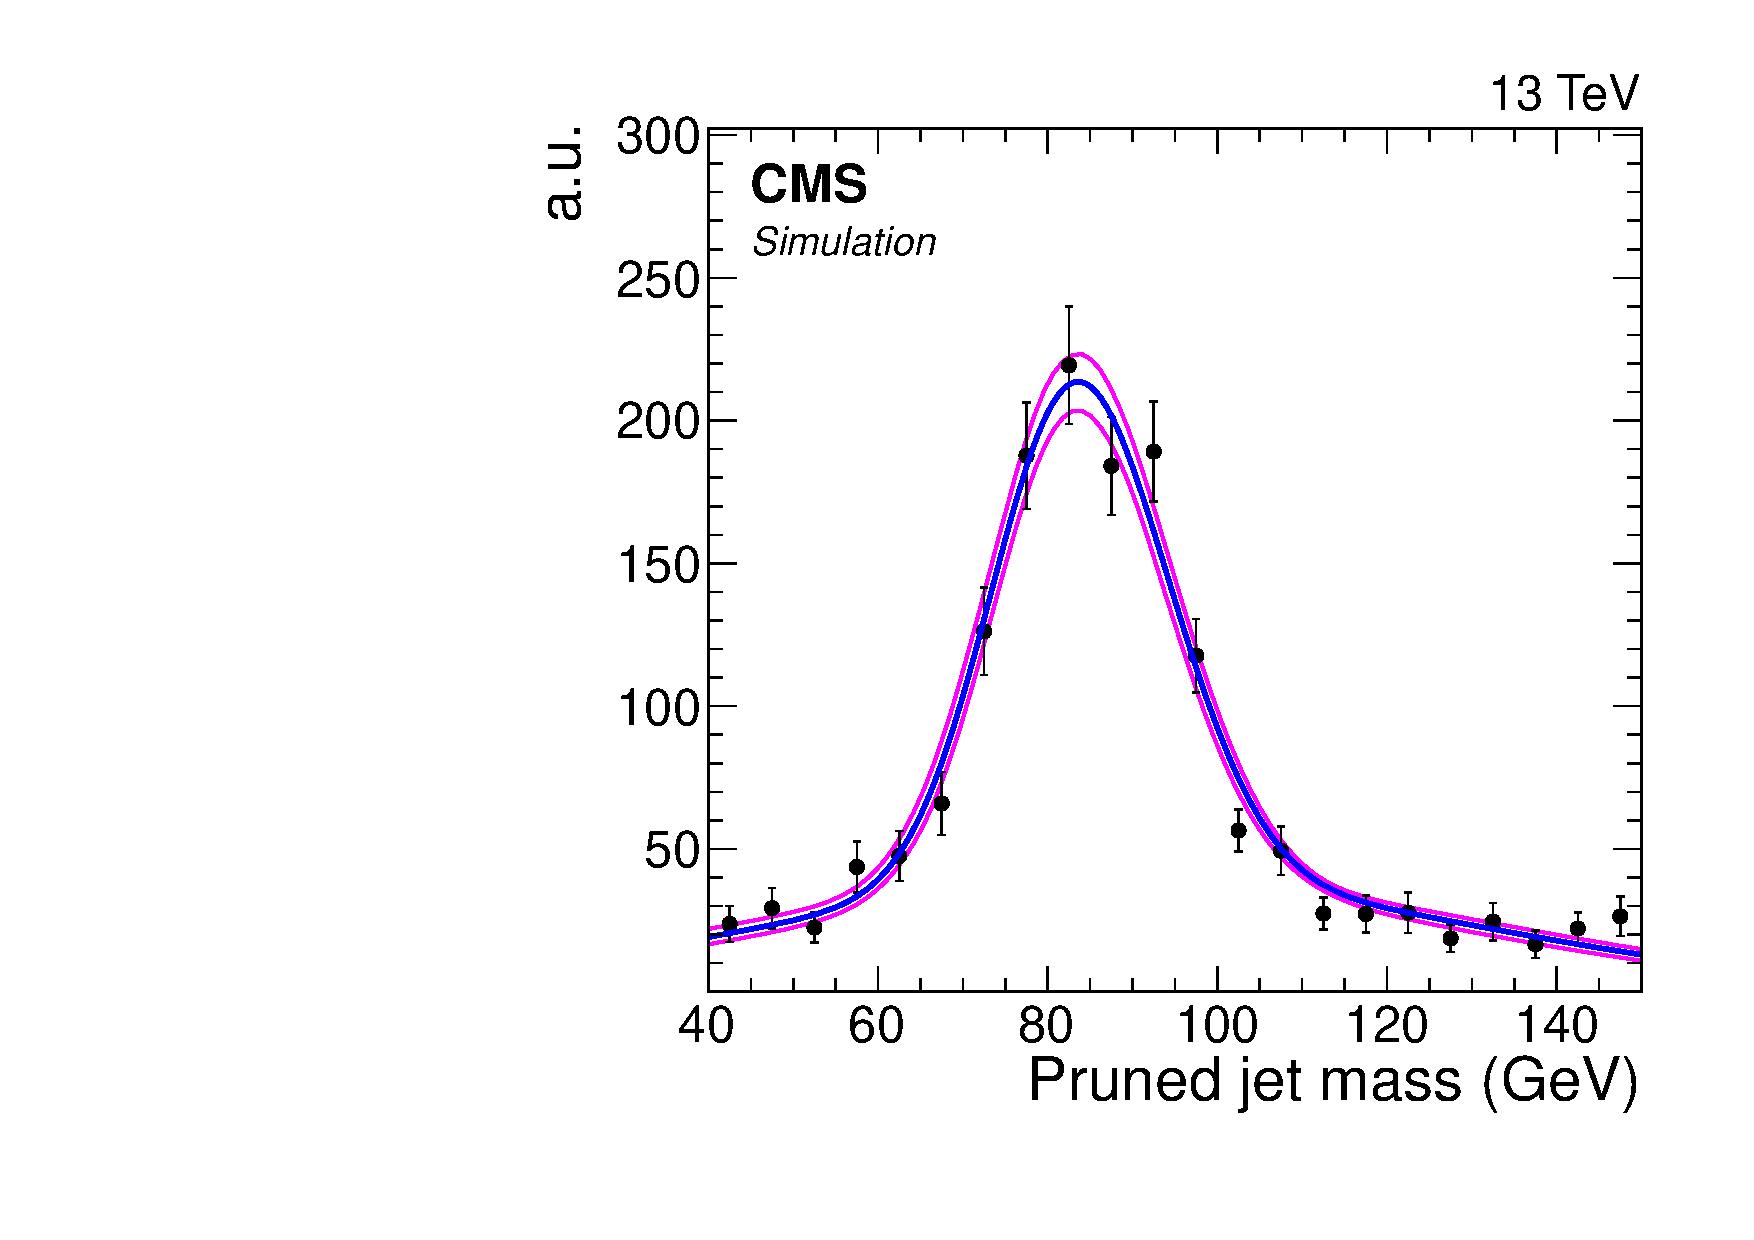
\includegraphics[width=0.45\textwidth]{\cheight/HP_mj_fitting-mu-VV.pdf}}
\caption{Functional forms describing the \mJ spectra for each background contribution after fitting the simulation data. (a) W+jets. (b) \ttbar. (c) Single top quark. (d) Diboson.}
\label{fig:mcfits_mj}
\end{figure}

The results of this fit procedure to extract the W+jets normalization are shown in Fig.~\ref{fig:mjfit8TeV} and~\ref{fig:mjfit13TeV}
for the $\ell\Pgn\bbbar$ and the $\ell\Pgn\qqbar$ channel, respectively.
The factors for correcting the simulated W-peak position and resolution to represent the observed data, taken from the top quark enriched control sample as described in Section~\ref{sec:vtagging}, are included in the \mJ spectra of Fig.~\ref{fig:mjfit13TeV}. 

\begin{figure}[!htb]
\centering     %%% not \center
\subfigure[]{\label{fig:mjfit8TeV_a}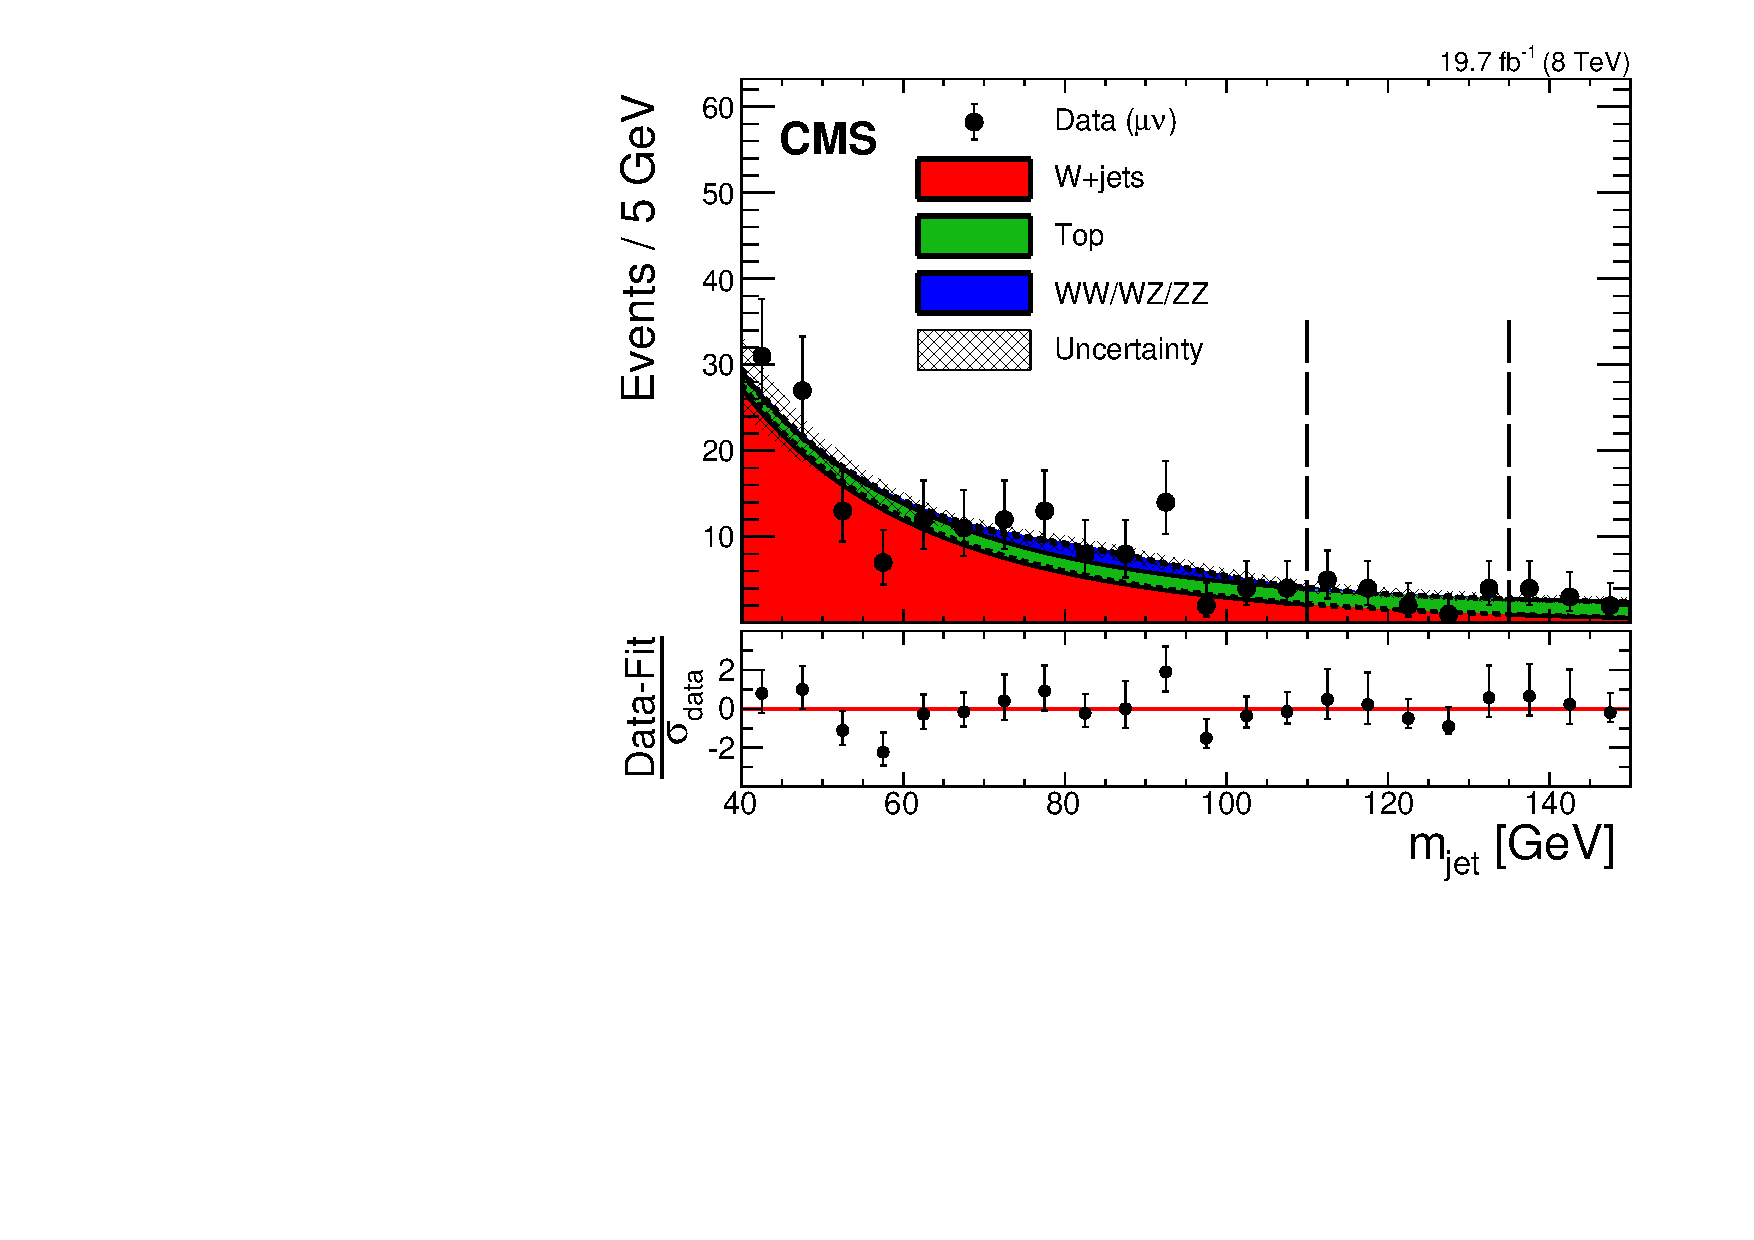
\includegraphics[width=0.45\textwidth]{\cheight/m_j_sideband_WJets0_MU_ALLP.pdf}}
\subfigure[]{\label{fig:mjfit8TeV_b}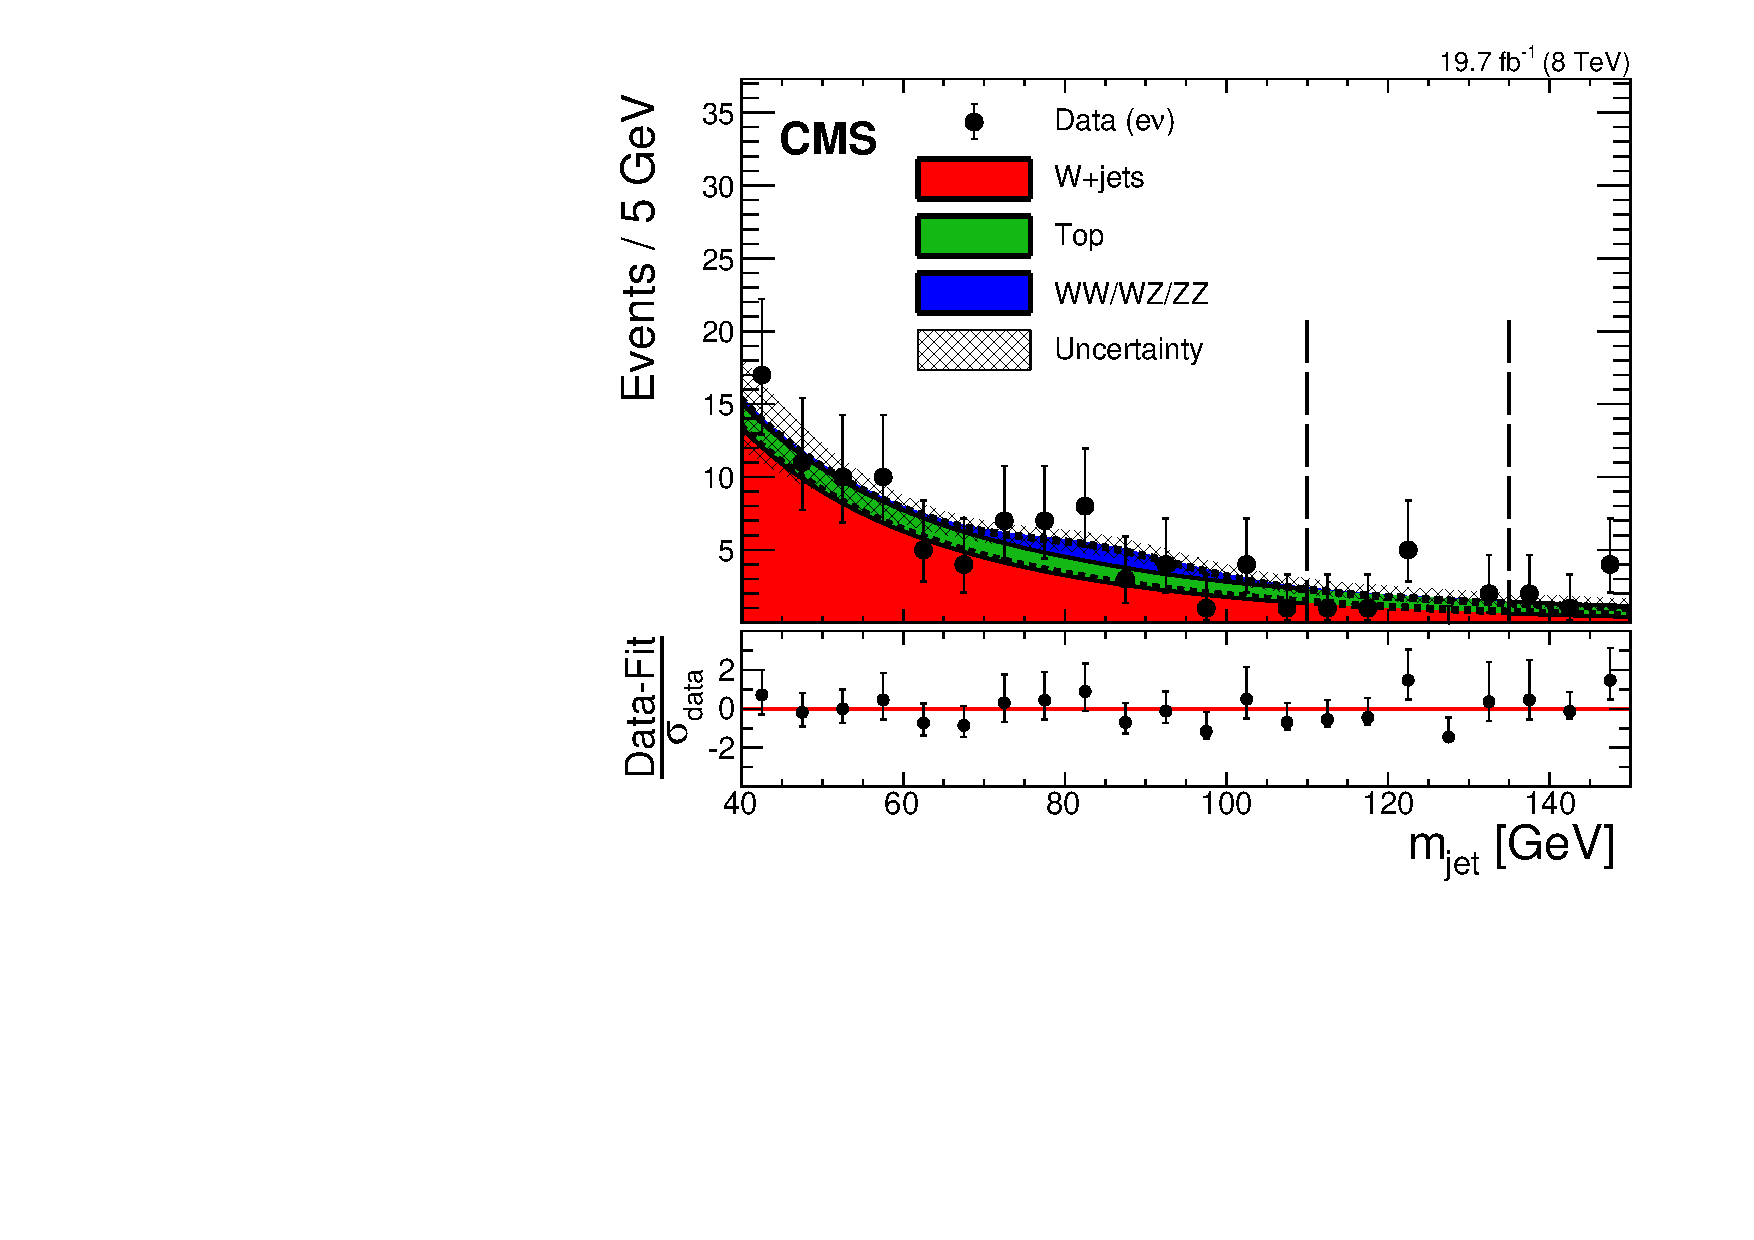
\includegraphics[width=0.45\textwidth]{\cheight/m_j_sideband_WJets0_ELE_ALLP.pdf}}
\caption{Distributions in pruned jet mass \mJ in the muon (a) and electron (b) channels for the $\ell\Pgn\bbbar$ analysis at 8\TeV. All selections are applied except the requirement on the \mJ signal window. The signal region lies between the dashed vertical lines. The hatched region indicates the statistical uncertainty of the fit. At the bottom of each plot, the bin-by-bin fit residuals, ($N_{\rm data}$ - $N_{\rm fit}$)/$\sigma_{\rm data}$, are shown.}
\label{fig:mjfit8TeV}
\end{figure}

\begin{figure}[!htb]
\centering     %%% not \center
\subfigure[]{\label{fig:mjfit13TeV_a}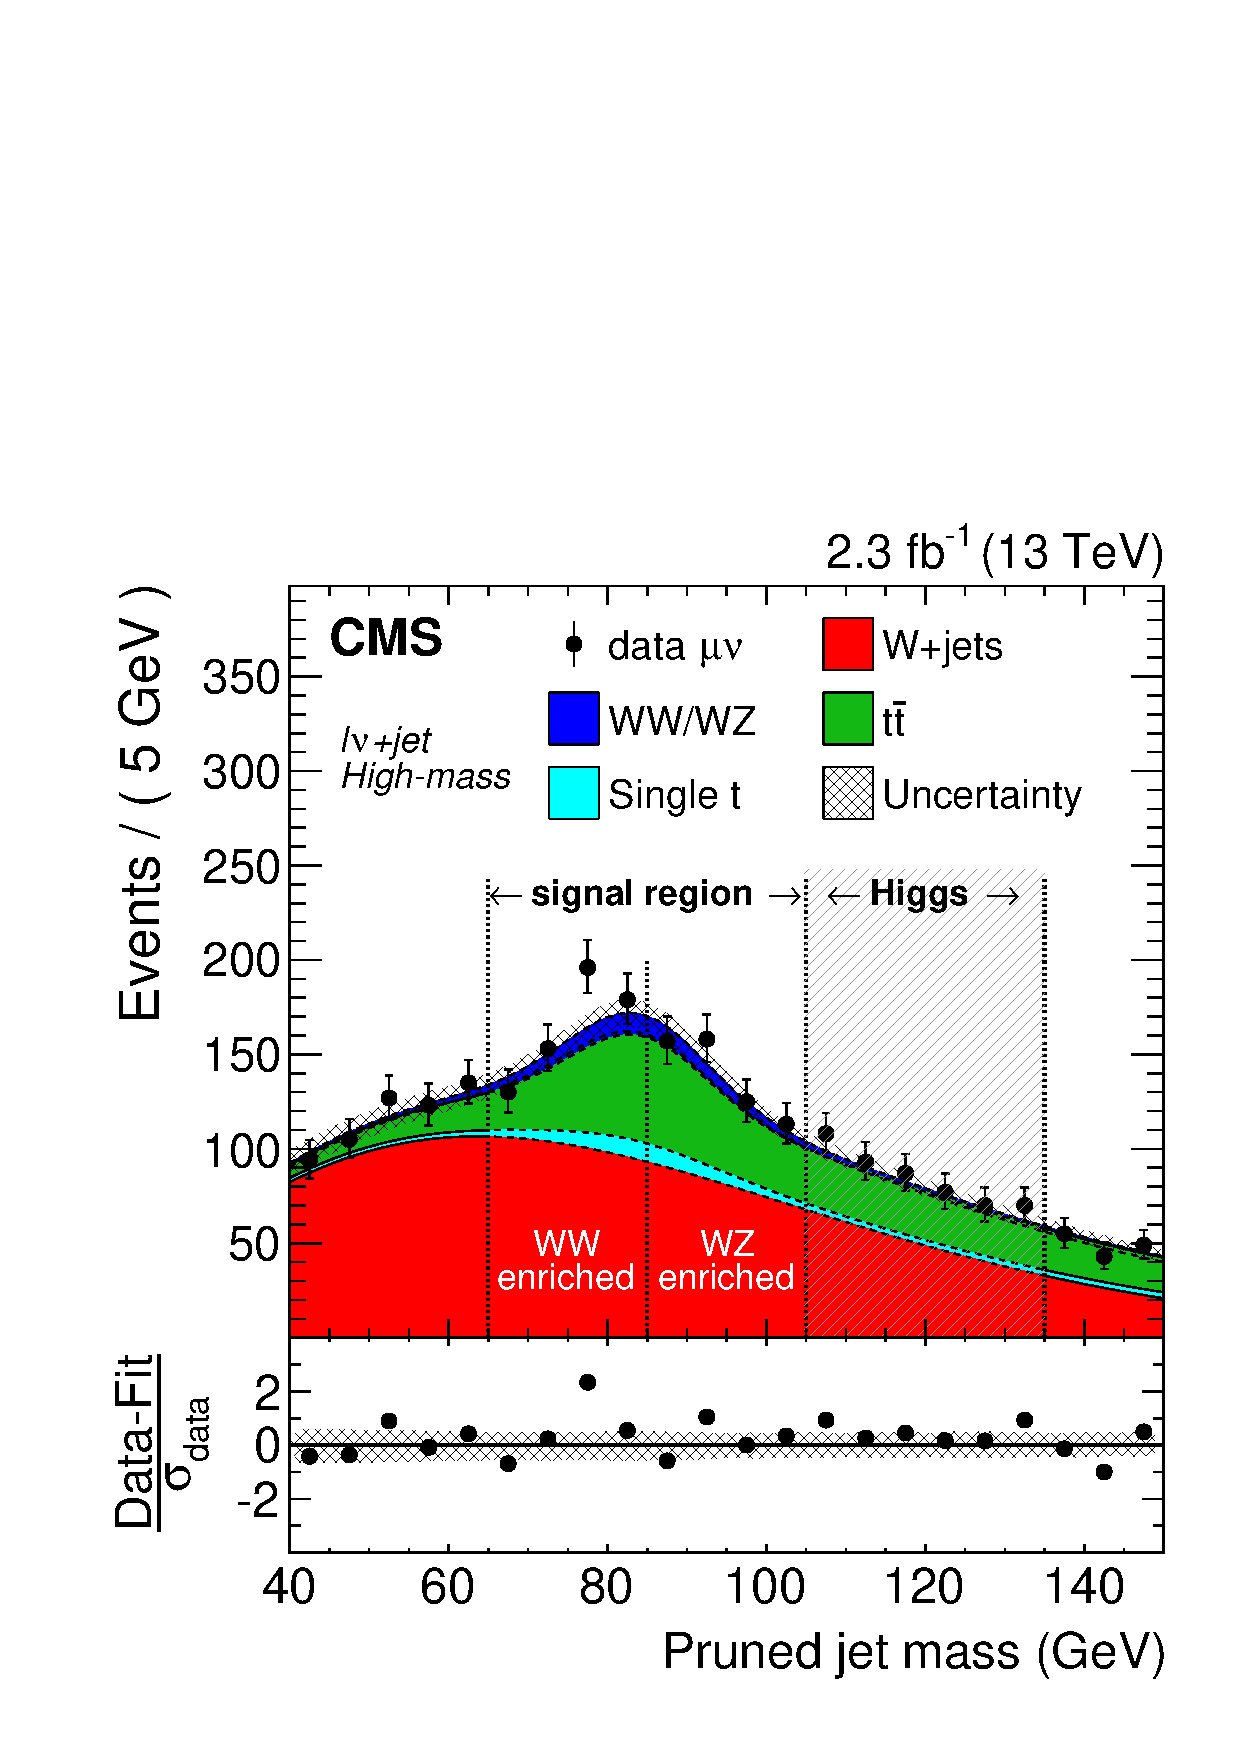
\includegraphics[width=0.45\textwidth]{\cheight/HP_mj_fitting-mu-m_j_sideband_WJets0_xww__with_pull.pdf}}
\subfigure[]{\label{fig:mjfit13TeV_b}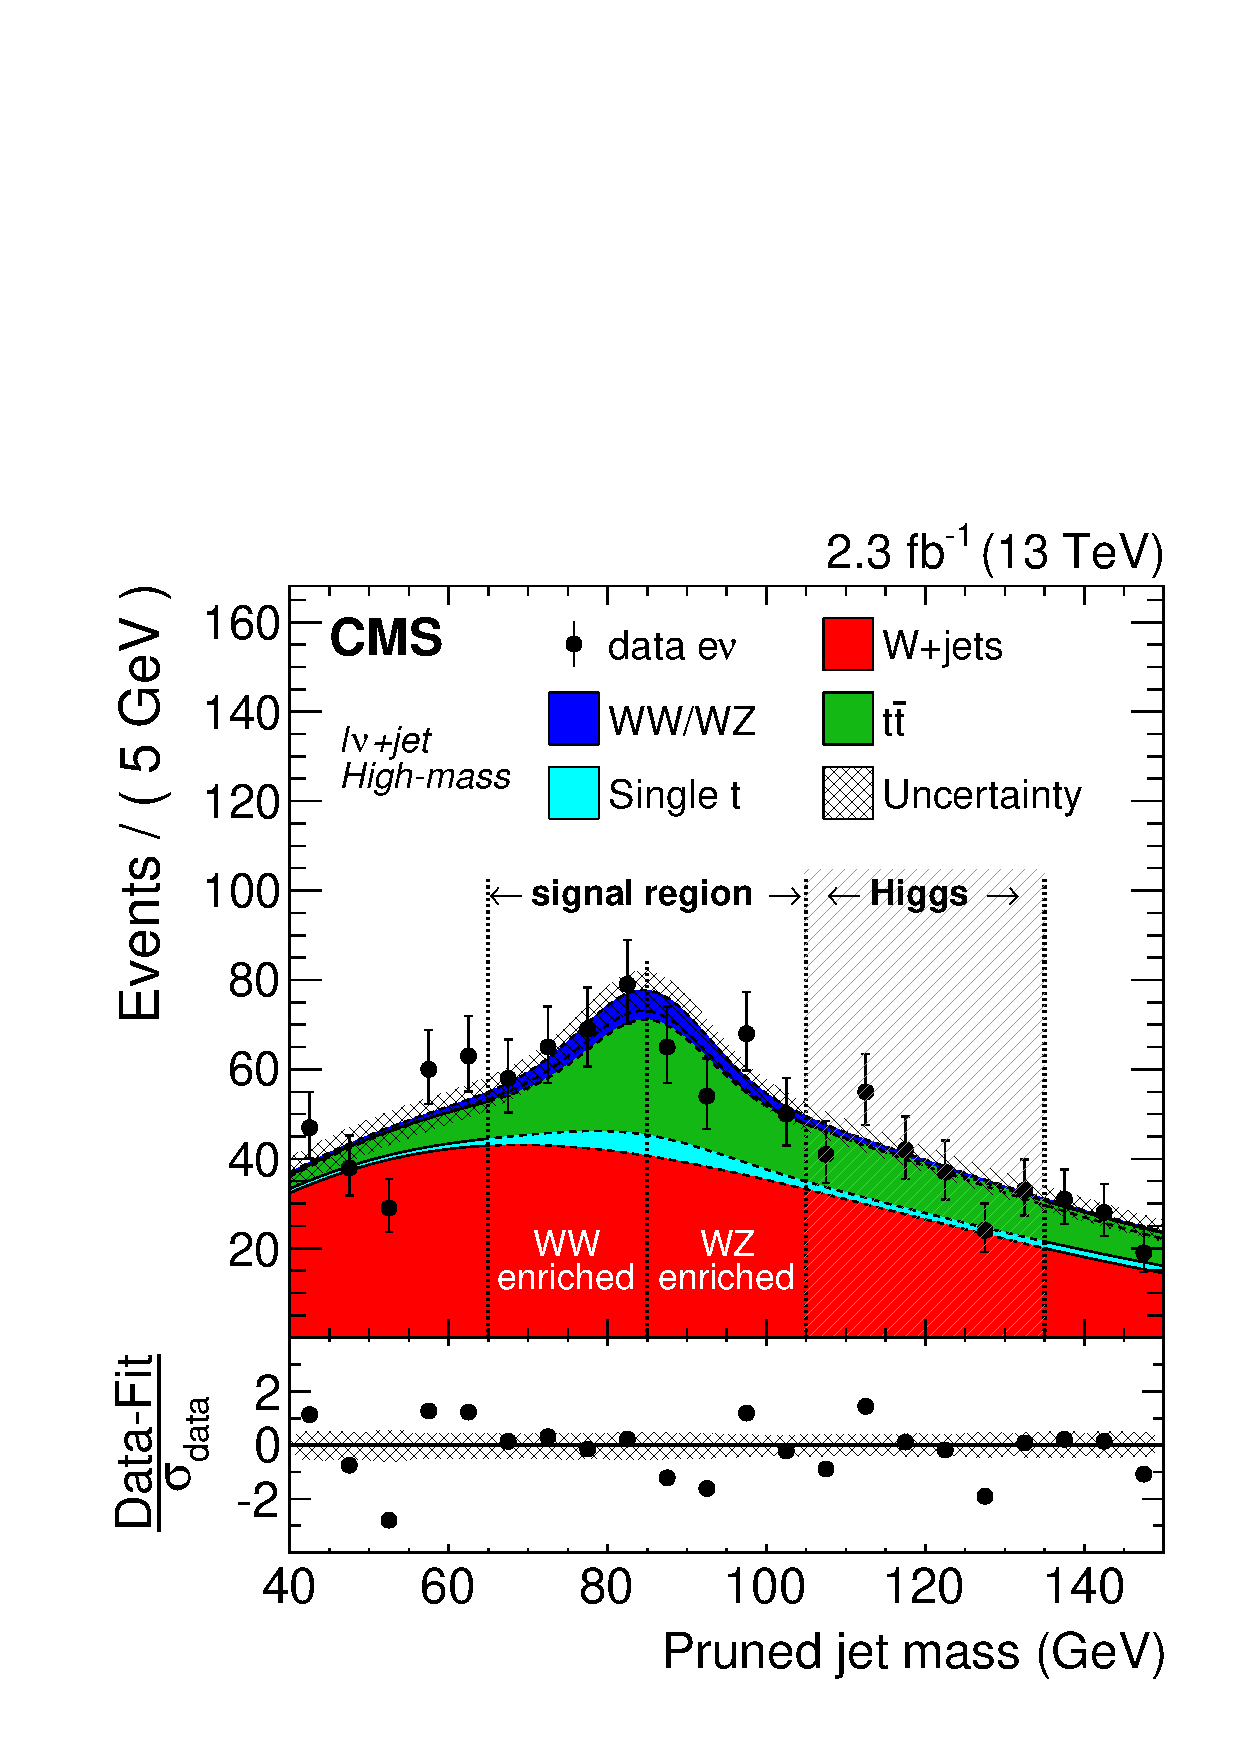
\includegraphics[width=0.45\textwidth]{\cheight/HP_mj_fitting-el-m_j_sideband_WJets0_xww__with_pull.pdf}}
\caption{Distributions in pruned jet mass in the muon (a) and electron (b) channels for the $\ell\Pgn\qqbar$ analysis at 13\TeV. All selections are applied except the requirement on the \mJ signal window. The signal regions and \mJ categories of the analysis are indicated by the vertical dotted lines. The shaded \mJ region 105--135\GeV is not used in the analysis. At the bottom of each plot, the bin-by-bin fit residuals, ($N_{\rm data}$ - $N_{\rm fit}$)/$\sigma_{\rm data}$, are shown together with the uncertainty band of the fit normalized by the statistical uncertainty of data, $\sigma_{\rm data}$.}
\label{fig:mjfit13TeV}
\end{figure}

%%%%%%%%%%%
\subsection{Extraction of the W+jets shape}~\label{subsec:wjetshape}
%%%%%%%%%%%

The form of the $\mlvj$ distribution for the W+jets background in the signal region (SR) is determined from the lower \mJ sideband, through the transfer function $\alpha_\mathrm{MC}(\mlvj)$ obtained from the W+jets simulation, and defined as:

\begin{equation}
\alpha_\mathrm{MC}(\mlvj) = \frac{F_\mathrm{MC, SR}^{\mathrm{W+jets}}(\mlvj)}{F_\mathrm{MC, SB}^{\mathrm{W+jets}}(\mlvj)},
\end{equation}

where $F_\mathrm{MC, SB}^{\mathrm{W+jets}}$ and $F_\mathrm{MC, SR}^{\mathrm{W+jets}}$ are the probability density functions used to describe the simulated \mlvj spectrum in the lower \mJ sideband and signal region, respectively.
The upper \mJ sideband is not considered since the W+jets shape is different here compared to what expected in the lower sideband. Furthermore, the upper sideband suffers from a larger \ttbar background contamination.

Since the lower sideband region does not represent a perfectly pure sample of W+jets events in data, the presence of minor backgrounds is subtracted from the observed diboson invariant mass distribution
to obtain an estimation of the W+jets contribution in the sideband control region of the data, $F_\mathrm{data, SB}^{\mathrm{W+jets}}(\mlvj)$.

The \mlvj range used in the estimate of the background distribution determines the region of masses probed by these searches.
This range is chosen to ensure a smoothly falling background spectrum, and therefore far enough from the kinematic turn-on at low masses generated by the acceptance selections,
allowing for a good stability and a robust control of the background estimation.
For this reason the low edge of the range is chosen at 0.7\TeV while the high edge is chosen such that it is not too far from the last value where data are still present.
Therefore, the fits are performed in the range $0.7 < \mlvj < 4\TeV$ for the 13\TeV analysis, while at 8\TeV no data are present above $\mlvj \approx 3\TeV$ and the the chosen range is therefore $0.7 < \mlvj < 3\TeV$.

To describe the smoothly falling W+jets background distribution, a parametrization of the form of a leveled exponential is adopted, defined as

\begin{equation}\label{eqn:mVVfunct}
   F_{\rm ExpTail}(x) = e^{-\frac{x}{a+bx}}.
\end{equation}

This functional form is found to adequately describe the simulation in both the signal region and the low sideband as demonstrated in Fig.~\ref{fig:mcfits_mlvj}. Tests are performed with alternative functional forms, and the background prediction is found to agree with the one of the default function within the uncertainties.
The minor background contributions are parametrized with a simple exponential functional form, except for the diboson contribution for which the $F_{\rm ExpTail}(x)$ defined above is used.

\begin{figure}[!htb]
\centering
\subfigure[]{\label{fig:mcfits_mlvj_a}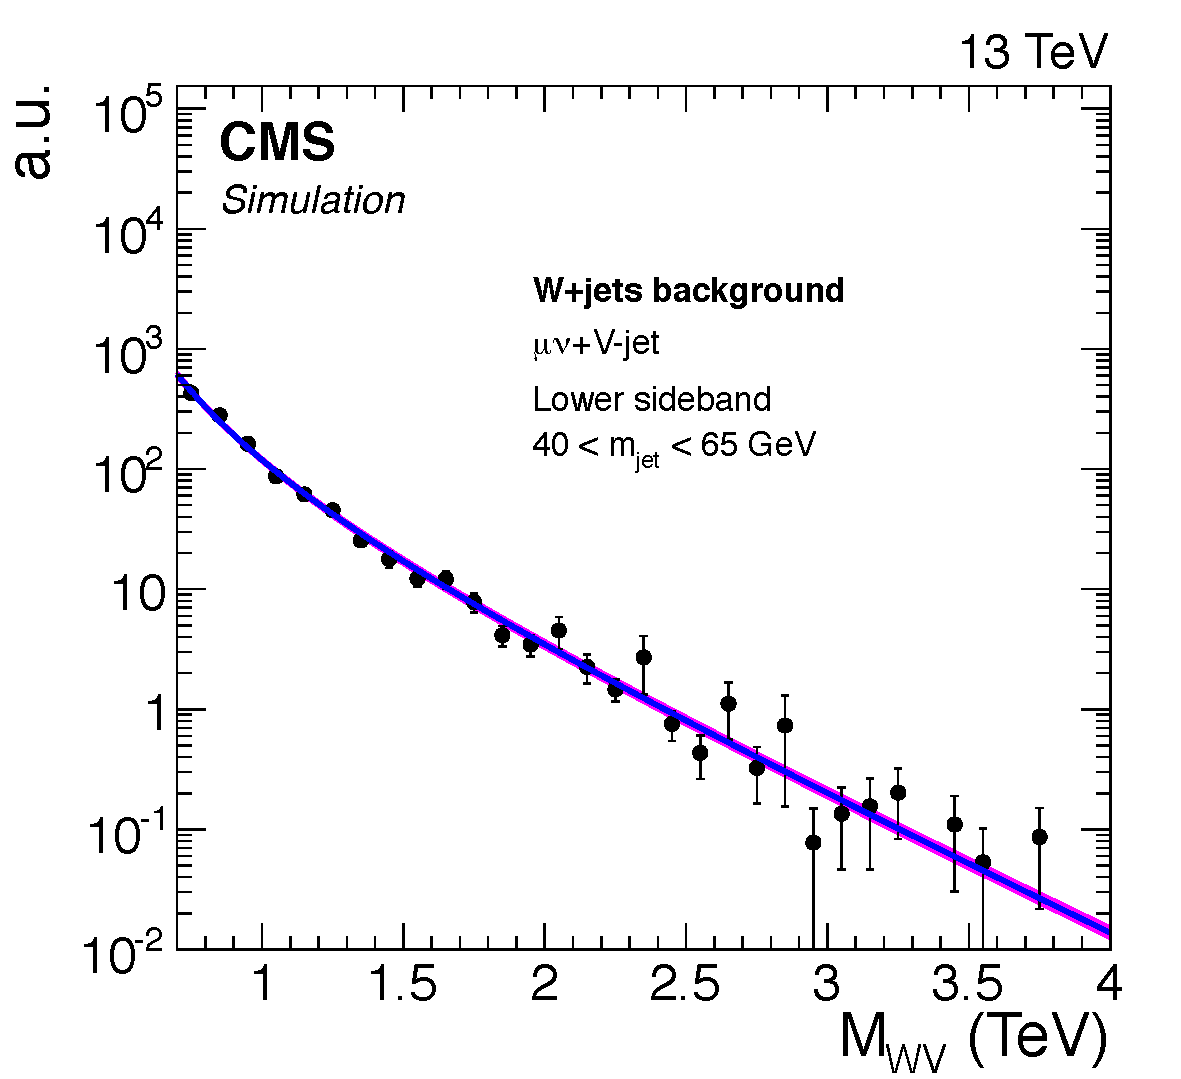
\includegraphics[width=0.32\textwidth]{\cheight/HP_mlvj_fitting_sb_lo-mu-WJets.pdf}}
\subfigure[]{\label{fig:mcfits_mlvj_b}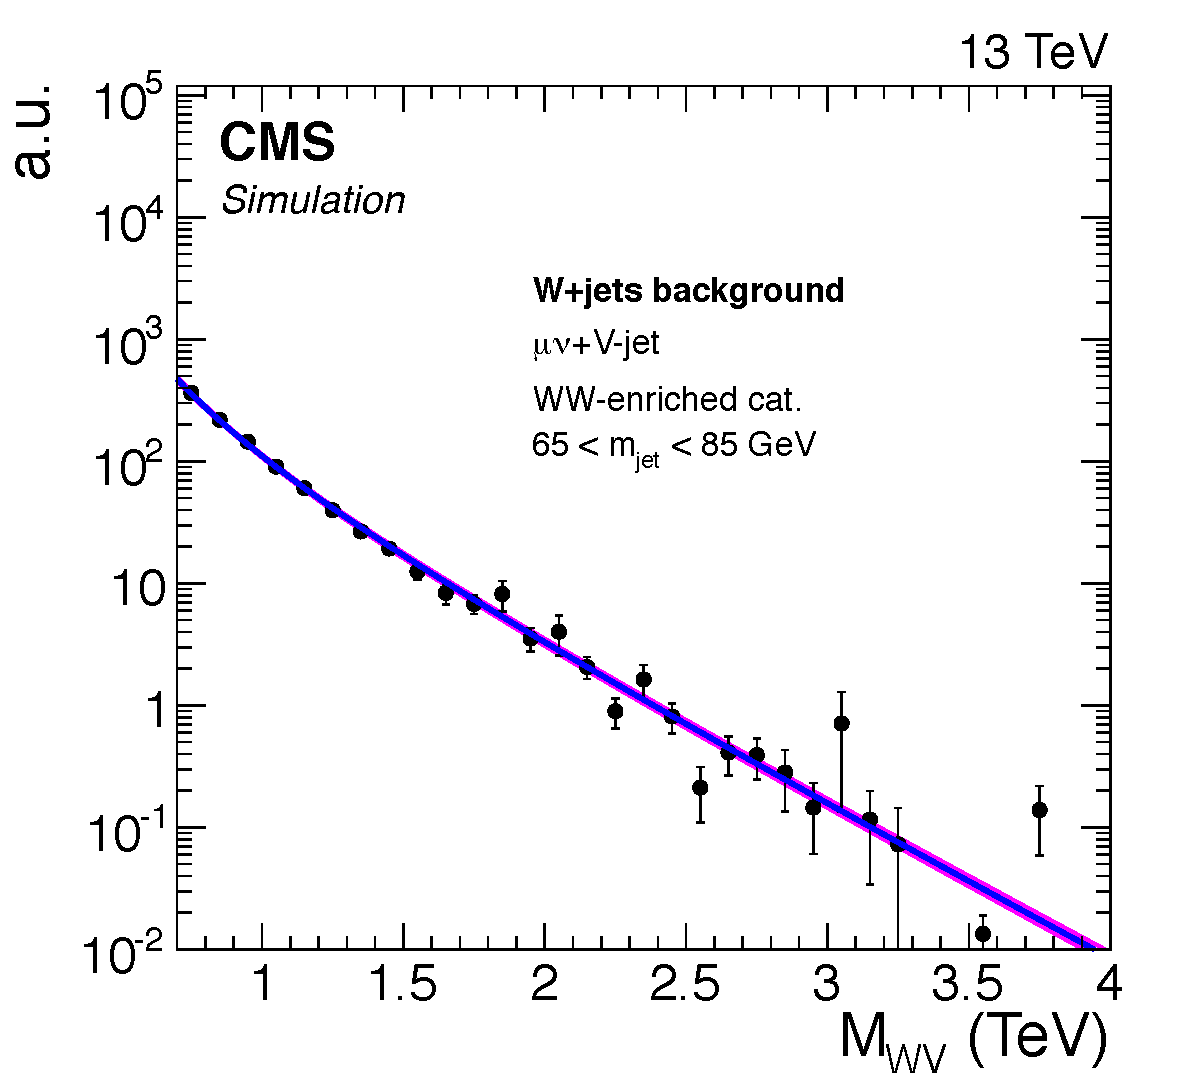
\includegraphics[width=0.32\textwidth]{\cheight/HPW_mlvj_fitting_signal_region-mu-WJets.pdf}}
\subfigure[]{\label{fig:mcfits_mlvj_c}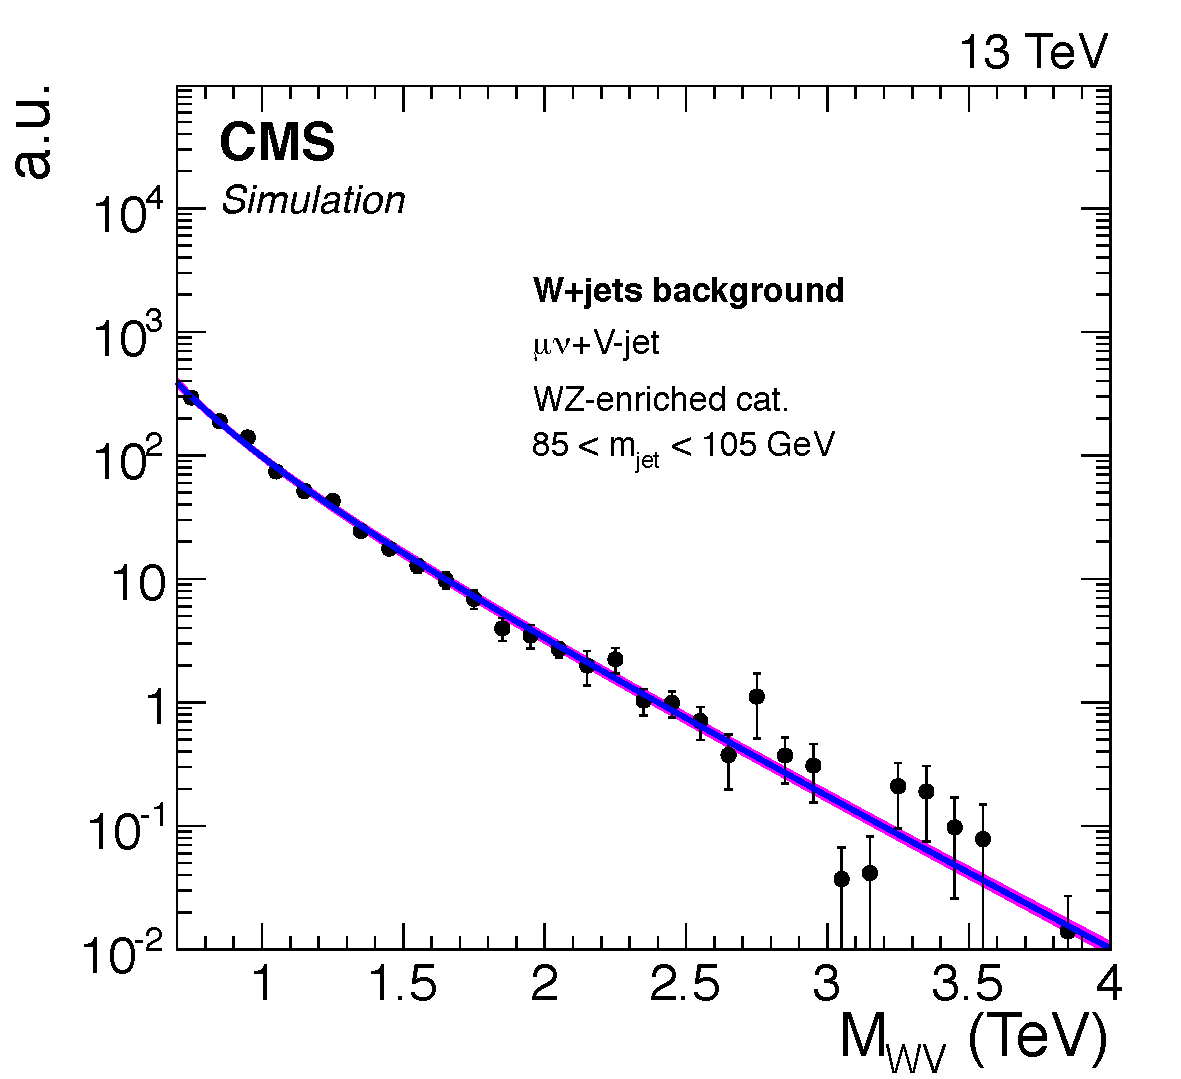
\includegraphics[width=0.32\textwidth]{\cheight/HPZ_mlvj_fitting_signal_region-mu-WJets.pdf}}
\caption{Functional form describing the diboson invariant mass spectrum of the W+jets background after fitting the simulation data. The distributions for the lower \mJ sideband (a), and the WW-enriched (b) and WZ-enriched (c) signal regions of the $\ell\nu\qqbar$ analysis are shown.}
\label{fig:mcfits_mlvj}
\end{figure}

For the $\ell\nu\qqbar$ analysis, the $\alpha_\mathrm{MC}$ is computed independently for the two WW- and WZ-enriched categories, which are therefore treated as two different signal regions.
Figure~\ref{fig:alphasWV_13TeV} shows the $\alpha_\mathrm{MC}$ for the two categories, obtained from a simultaneous fit of W+jets simulated data in the lower sideband and in the signal region defined by the category using the parametrization in Eq.~\ref{eqn:mVVfunct}.
The blue and the red lines represent the probability density functions describing the W+jets background with \mJ in the lower sideband and signal region, respectively, and given by the leveled-exponential function of Eq.~\ref{eqn:mVVfunct}. A simultaneous fit is performed of the two distributions, where the parameters used to model the distribution in the signal region are correlated with the ones used to model the distribution in the sideband.
The transfer function $\alpha_\mathrm{MC}$  is shown as a solide black line, while the dark (light) shaded region corresponds to the 1$\sigma$ (2$\sigma$) statistical uncertainty of the fit.
These uncertainties only represent the uncertainty in the modelling of the W+jets distribution. The bands have a size of approximately zero around 2\TeV as the $\alpha_\mathrm{MC}$ is the ratio of two probability density functions which have to cross in order to conserve the total probability. Similar results are obtained for the $\ell\Pgn\bbbar$ analysis.

\begin{figure}[!htb]
\centering
\subfigure[]{\label{fig:alphasWV_13TeV_a}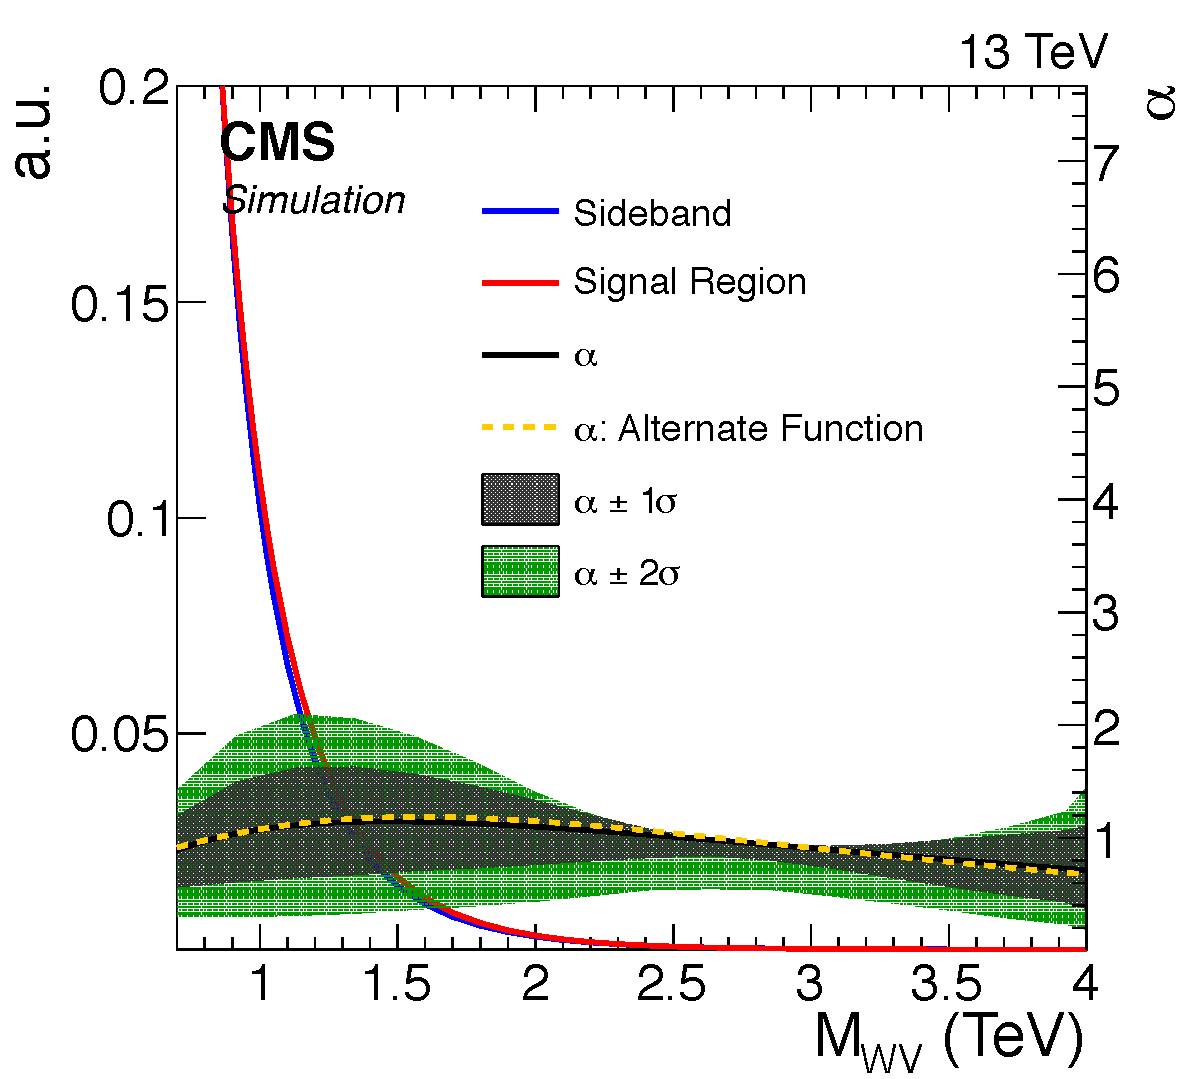
\includegraphics[width=0.45\textwidth]{\cheight/alpha_HPW-mu.pdf}}
\subfigure[]{\label{fig:alphasWV_13TeV_b}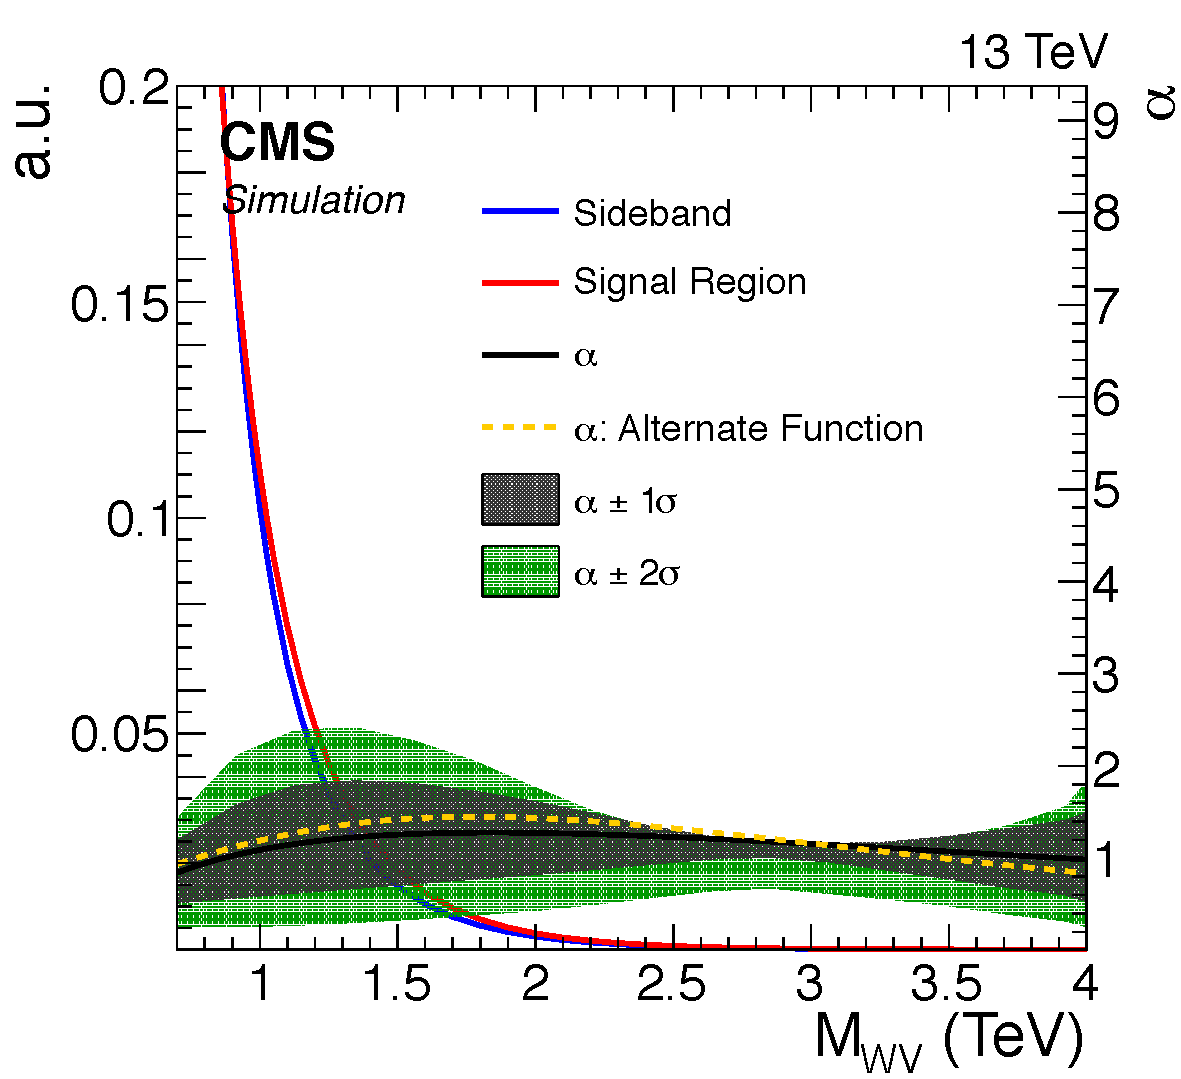
\includegraphics[width=0.45\textwidth]{\cheight/alpha_HPZ-mu.pdf}}
\caption{The transfer functions $\alpha_\mathrm{MC}$ from the lower \mJ sideband to the signal region defined by the WW-enriched (a) and WZ-enriched (b) category of the $\ell\nu\qqbar$ analysis. The dark and light shaded areas represent the statistical uncertainty of the fit. The blue and the red lines represents the probability density functions describing the W+jets background with \mJ in the lower sideband and signal region, respectively. The $\alpha_\mathrm{MC}$ obtained fitting the W+jets with and alternative function is shown as yellow line.}
\label{fig:alphasWV_13TeV}
\end{figure}

In Fig.~\ref{fig:sbfitmlvj13TeV}, the result of the fit to the \mlvj distribution of the data with \mJ in the lower sideband is shown for the electron and muon channels of the $\ell\Pgn\qqbar$ analysis.
From this fit, an estimation of $F_\mathrm{data, SB}^{\mathrm{W+jets}}(\mlvj)$ is obtained.
Finally, the W+jets background distribution in the signal region is then extrapolated by rescaling $F_\mathrm{data, SB}^{\mathrm{W+jets}}$ by $\alpha_\mathrm{MC}$.
The minor backgrounds are then added to the W+jets background to obtain the total SM prediction in the signal region, which is given by

\begin{equation}\label{eqn:alpha_totalBkg}
\footnotesize
N_\mathrm{SR}^\mathrm{bkg}(\mlvj) = N_\mathrm{SR}^\mathrm{W+jets} \times \alpha_\mathrm{MC}(\mlvj) \times F_\mathrm{data, SB}^{\mathrm{W+jets}}(\mlvj) + \sum_{k} N_\mathrm{SR}^k \times F_\mathrm{MC,SR}^k(\mlvj).
\end{equation}

In the above equation, the sum runs over the products of the normalization $N_\mathrm{MC,SR}^k$ and probability density function $F_\mathrm{MC,SR}^k$ of each minor background contribution $k$, while $N_\mathrm{SR}^\mathrm{W+jets}$ and $F_\mathrm{data, SB}^{\mathrm{W+jets}}$ represent the normalization and probability density function of the W+jets background derived from data as described previously in this chapter. The transfer function $\alpha_\mathrm{MC}$ accounts for small kinematic differences between the signal and the sideband regions.

Results of the final background extraction in the signal region will be presented in Chapters~\ref{ch:results8} and~\ref{ch:results13} or the $\ell\Pgn\bbbar$ and $\ell\Pgn\qqbar$ analysis, respectively.

\begin{figure}[!htb]
\centering
\subfigure[]{\label{fig:sbfitmlvj13TeV_a}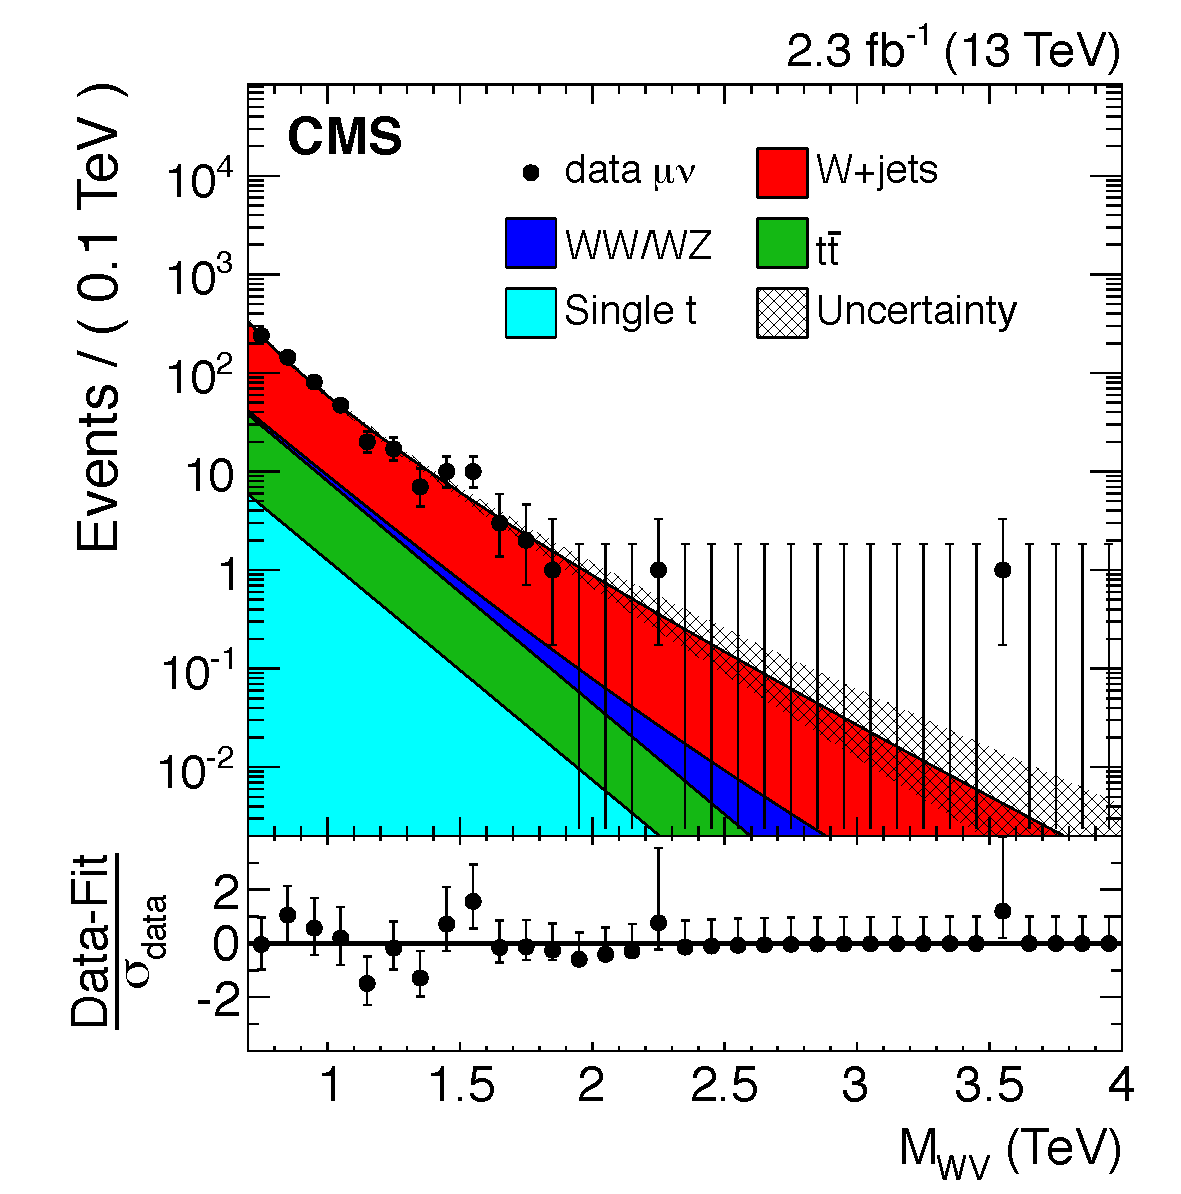
\includegraphics[width=0.45\textwidth]{\cheight/HP_m_lvj_sb_lo-mu.pdf}}
\subfigure[]{\label{fig:sbfitmlvj13TeV_b}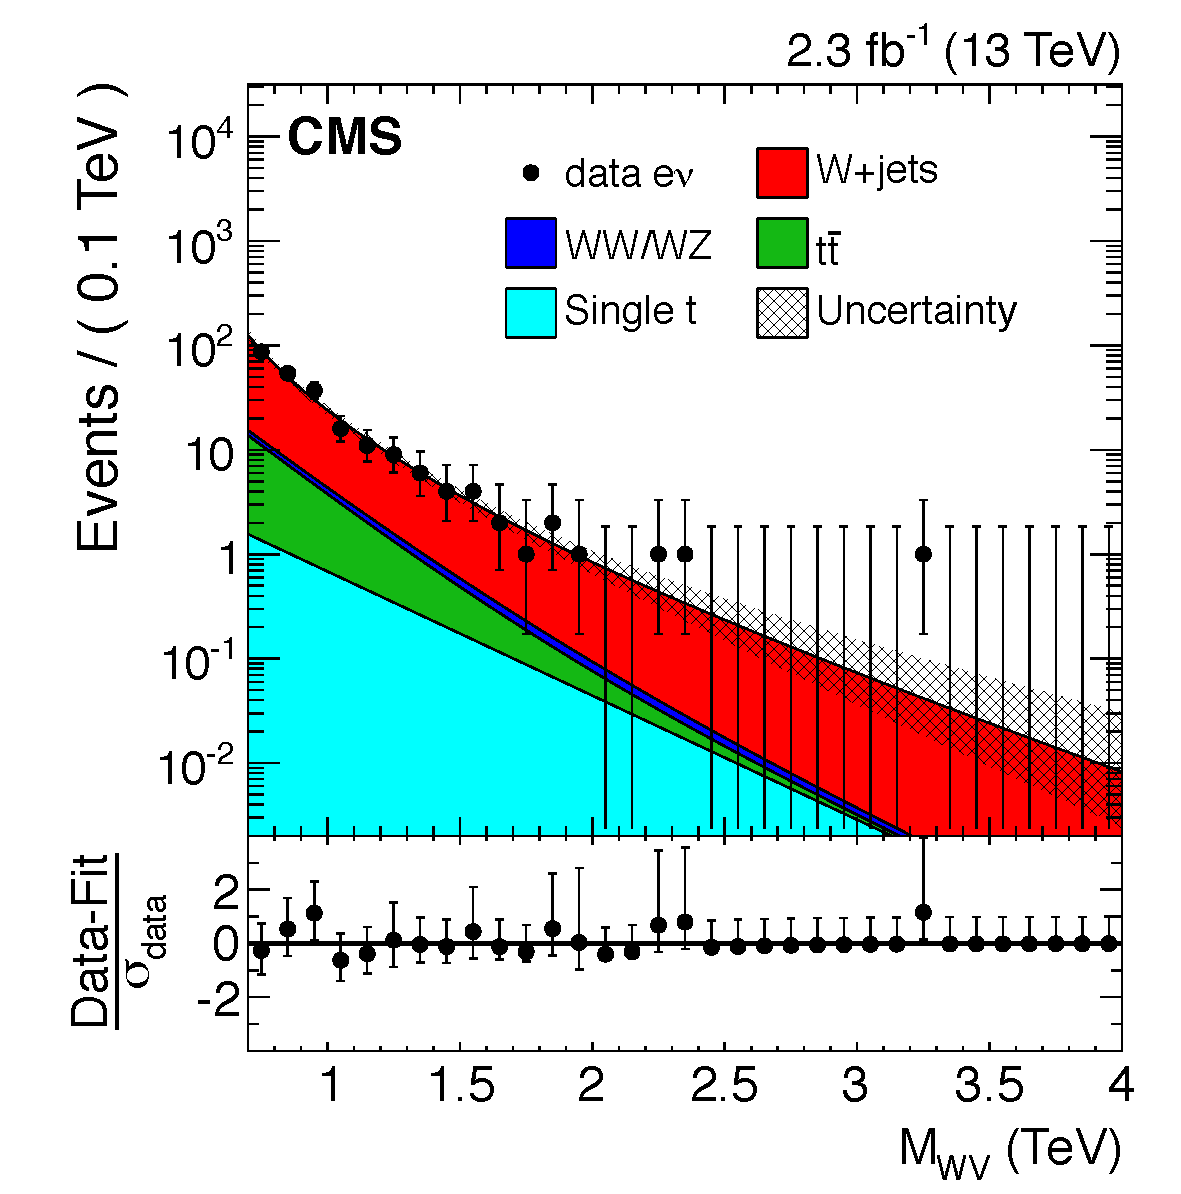
\includegraphics[width=0.45\textwidth]{\cheight/HP_m_lvj_sb_lo-el.pdf}}
\caption{Results of the fit to the \mWV distribution of the data with \mJ in the lower sideband to estimate $F_\mathrm{data, SB}^{\mathrm{W+jets}}$ for both muon (a) and electron (b) channels of the $\ell\Pgn\qqbar$ analysis. Minor backgrounds are estimated from simulation, while the W+jets contribution is the result of the fit to the data.}
\label{fig:sbfitmlvj13TeV}
\end{figure}

%%%%%%%%%%%
\subsection{Validation of the $\alpha$ method}
%%%%%%%%%%%

To test the validity and the robustness of the data driven method used to estimate the W+jets contribution and described previously in this section, a closure test is performed.
In this test, the background is extracted to a signal free control region that allows to check the compatibility with data for both the distribution and normalization.
In order to achieve this, the low mass sideband defined in Table~\ref{tab:sidebands} is divided into two regions:
$40 < \mJ < 55\GeV$, referred to as ``region A'', is used as sideband, while $55 < \mJ < 65\GeV$, referred to as ``region B'', is used as signal region.
The W+jets background normalization is then predicted in region B by performing a fit to the \mJ distribution of the data in region A and in the upper sideband (Table~\ref{tab:sidebands}),
while its distribution in \mlvj is extrapolated in region B with a fit of the data in region A and a suitable transfer function $\alpha_\mathrm{MC}$.
In this test, the $\alpha_\mathrm{MC}$ is defined as the ratio between the simulated W+jets background distributions in \mlvj in region B and A.
%The W+jets background normalization and \mlvj distribution is predicted in region B by performing a fit of the data in region A, following the procedure described previously in this section.

An example of the result of this test is presented in the following for the muon channel in the $\ell\nu\qqbar$ analysis.
Figure~\ref{fig:mj_closureTest} shows the results of the fit to the \mJ distribution of the data inside the region A and the HSB, performed to extract the expected W+jets normalization inside the region B.

\begin{figure}[!htb]
\centering
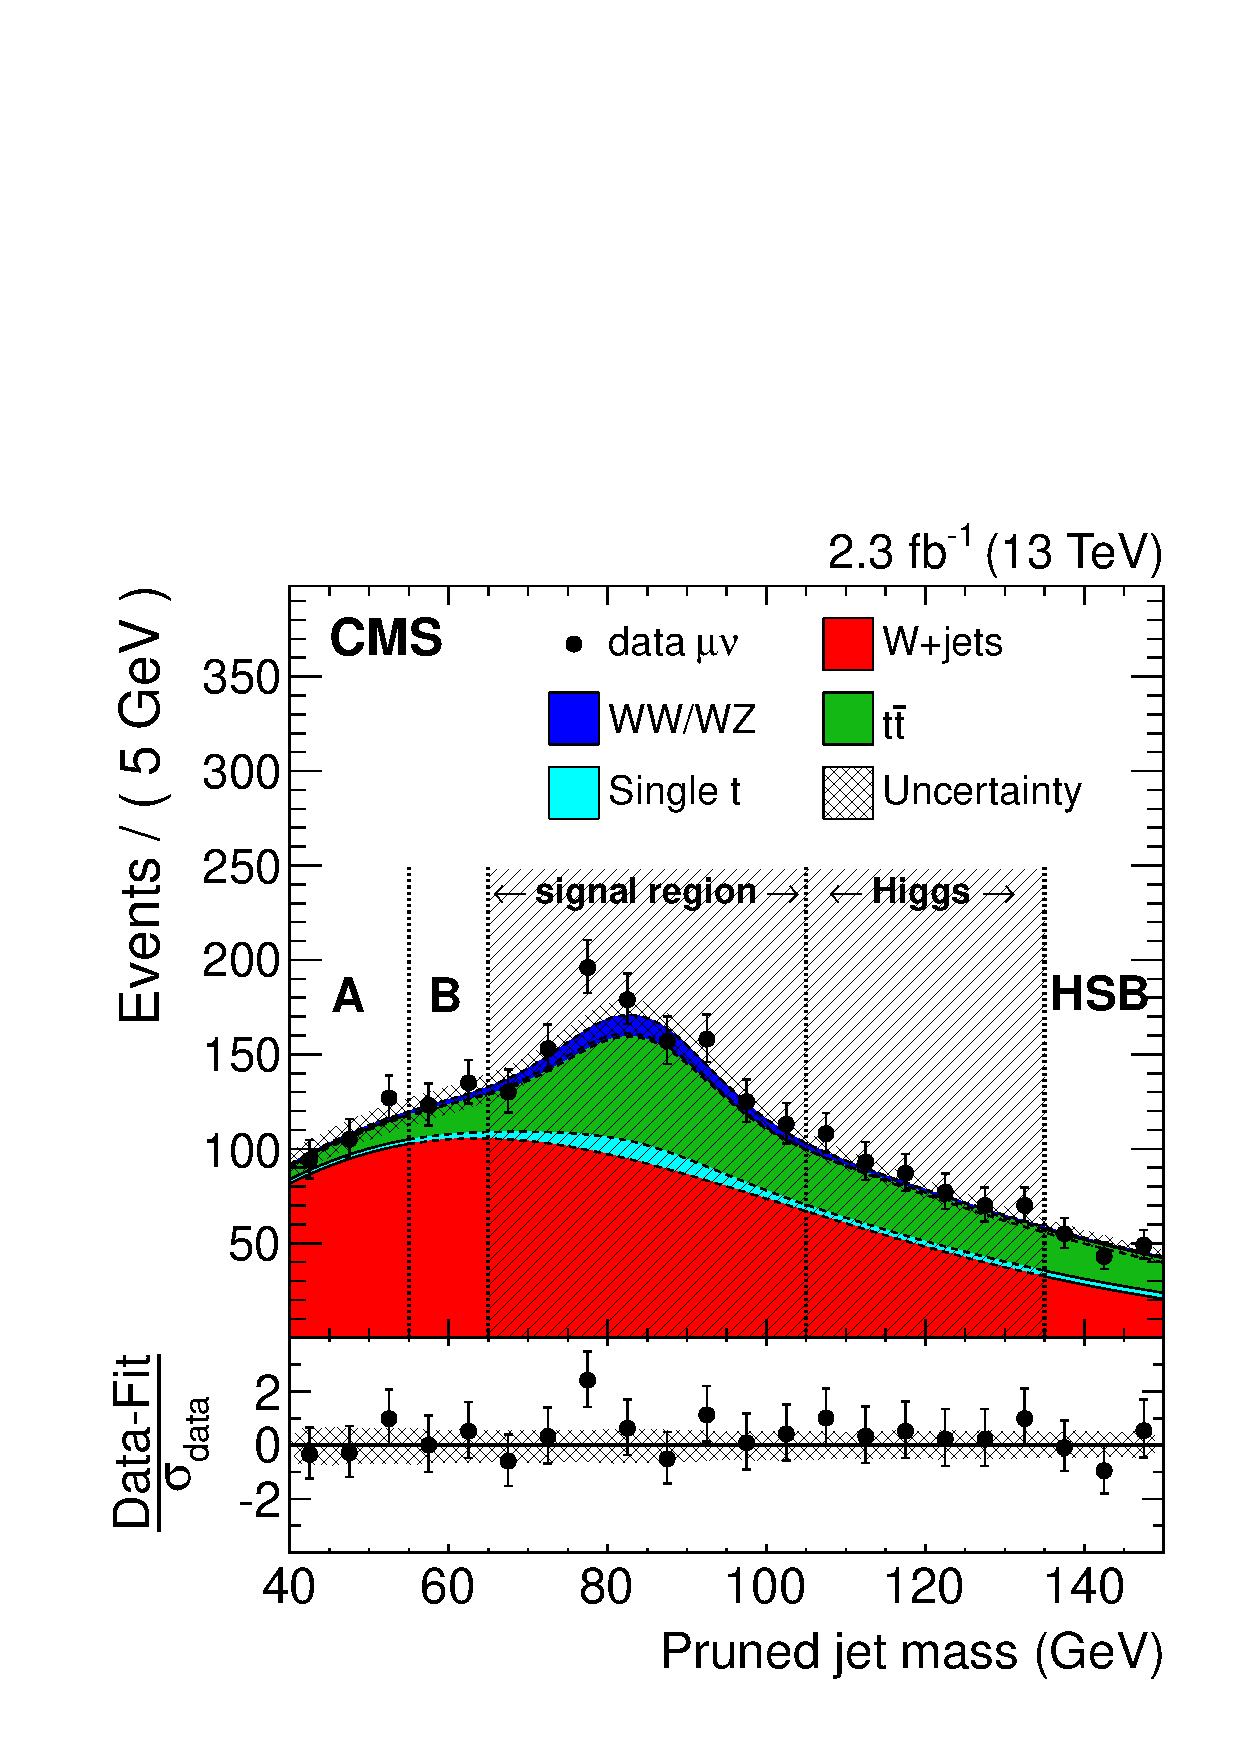
\includegraphics[width=0.5\textwidth]{\cheight/closureTest_HP_mu_mjetpruned.pdf}
\caption{Result of the closure test for the muon channel in the $\ell\nu\qqbar$ analysis. The plot shows the fit to the pruned jet mass distribution considering only events in data with \mJ in the ranges 40--55\GeV (A) and 135--150\GeV (HSB) performed to extract the W+jets normalization inside region B.}
\label{fig:mj_closureTest}
\end{figure}

Figure~\ref{fig:mlvjSBandAlpha_closureTest_a} shows the transfer function $\alpha_\mathrm{MC}$ obtained from a simultaneous fit of W+jets simulated events in the region A and in the region B, using the leveled-exponential parametrization defined in Eq.~\ref{eqn:mVVfunct}. In Fig.~\ref{fig:mlvjSBandAlpha_closureTest_b}, the result of the fit to the \mlvj distribution of the data with \mJ in the lower sideband is shown, where the W+jets shape is modelled through the same leveled-exponential function.

\begin{figure}[!htb]
\centering
\subfigure[]{\label{fig:mlvjSBandAlpha_closureTest_a}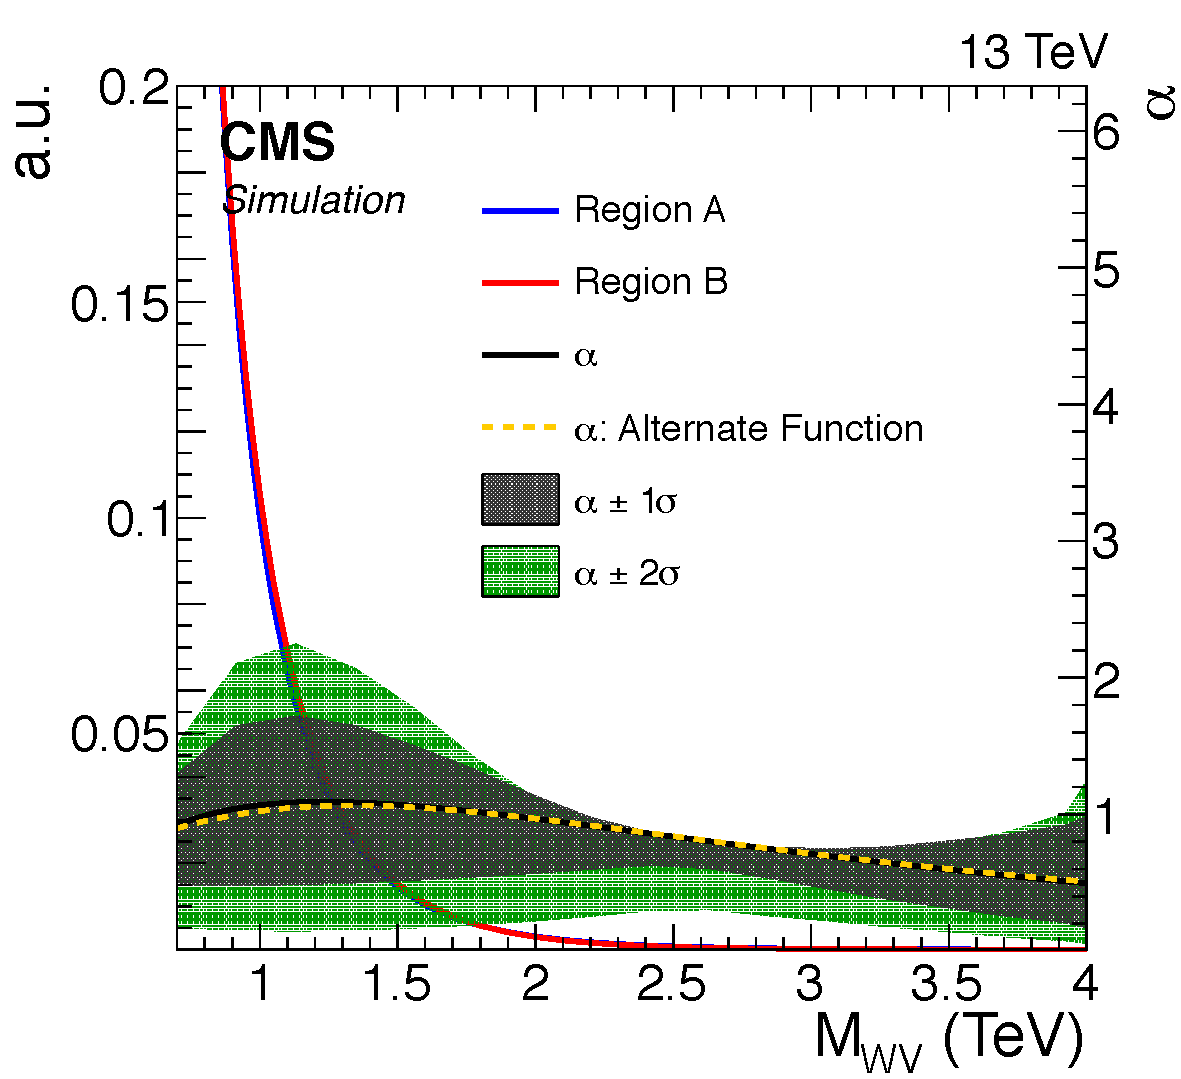
\includegraphics[width=0.47\textwidth]{\cheight/closureTest_HP_mu_alpha.pdf}}
\subfigure[]{\label{fig:mlvjSBandAlpha_closureTest_b}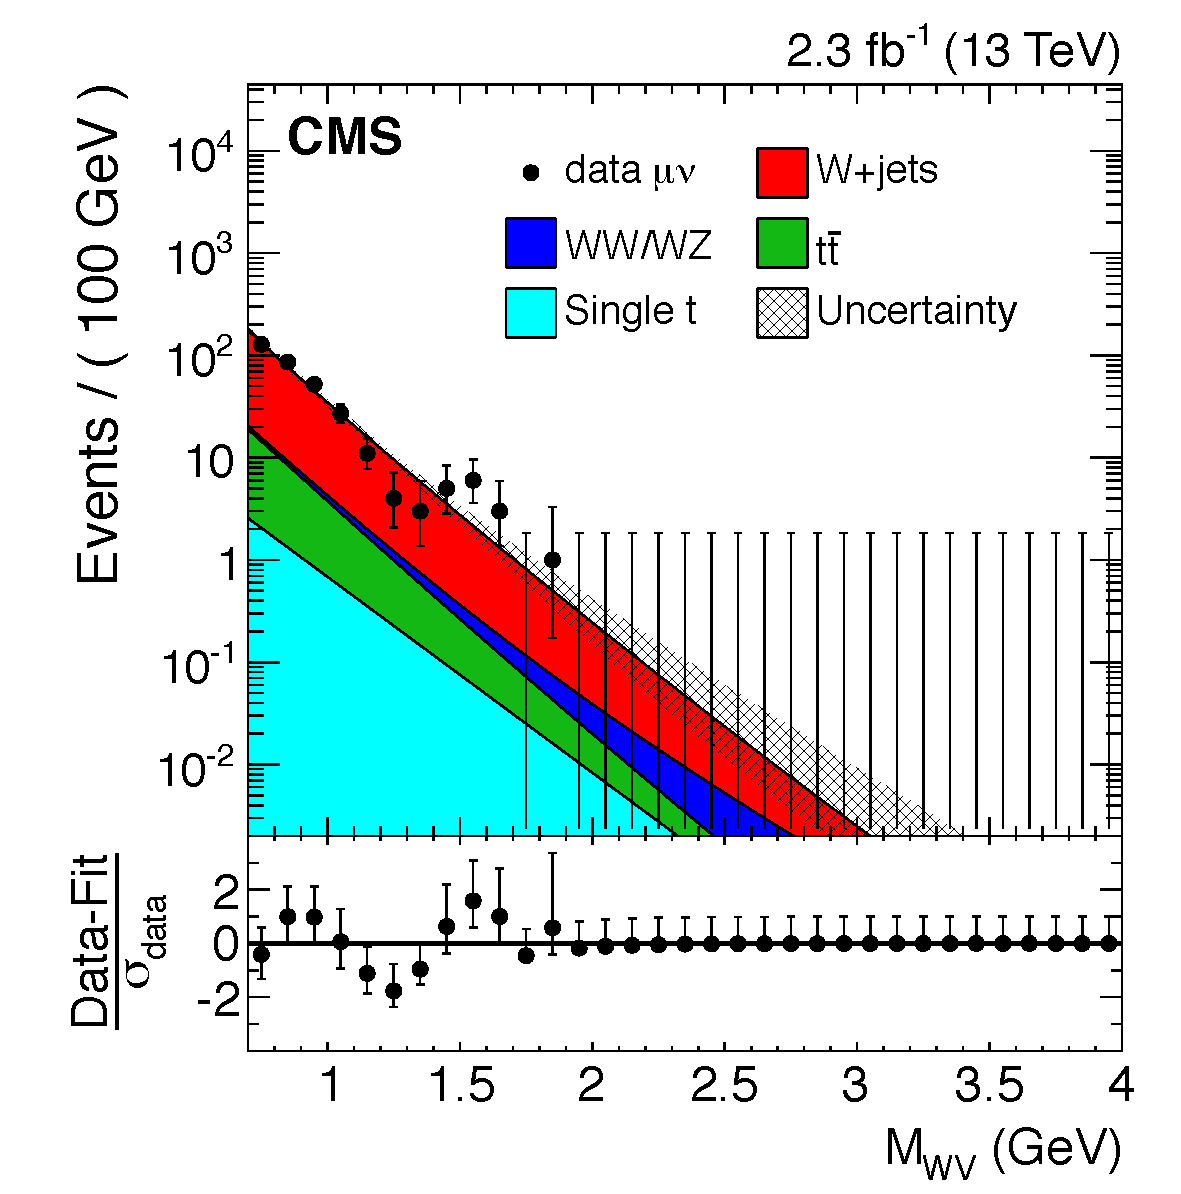
\includegraphics[width=0.43\textwidth]{\cheight/closureTest_HP_mu_regionA_mlvj.pdf}}
\caption{(a) The transfer function $\alpha_\mathrm{MC}$ obtained by simultaneously fitting the diboson invariant mass distributions of simulation data inside the sideband (A) and signal region (B). (b) Diboson invariant mass distribution for events with $40 < \mJ < 55\GeV$ (A). The W+jets shape is fitted, after subtracting contaminations from minor backgrounds, by means of a leveled-exponential function.}
\label{fig:mlvjSBandAlpha_closureTest}
\end{figure}

Finally, Fig.~\ref{fig:mlvjSR_closureTest} shows a comparison between the total predicted background, obtained through Eq.~\ref{eqn:alpha_totalBkg}, and the data inside the signal free region B.
A good agreement is found over the whole \mlvj range.
The test has been performed for both lepton flavours for the $\ell\nu\qqbar$ analysis, as well as for the $\ell\nu\bbbar$ analysis where slightly different definitions for region A and B are used.
In all the cases, consistency between the predicted background and the data is observed, thus validating the proposed strategy for the W+jets background estimation.

\begin{figure}[!htb]
\centering
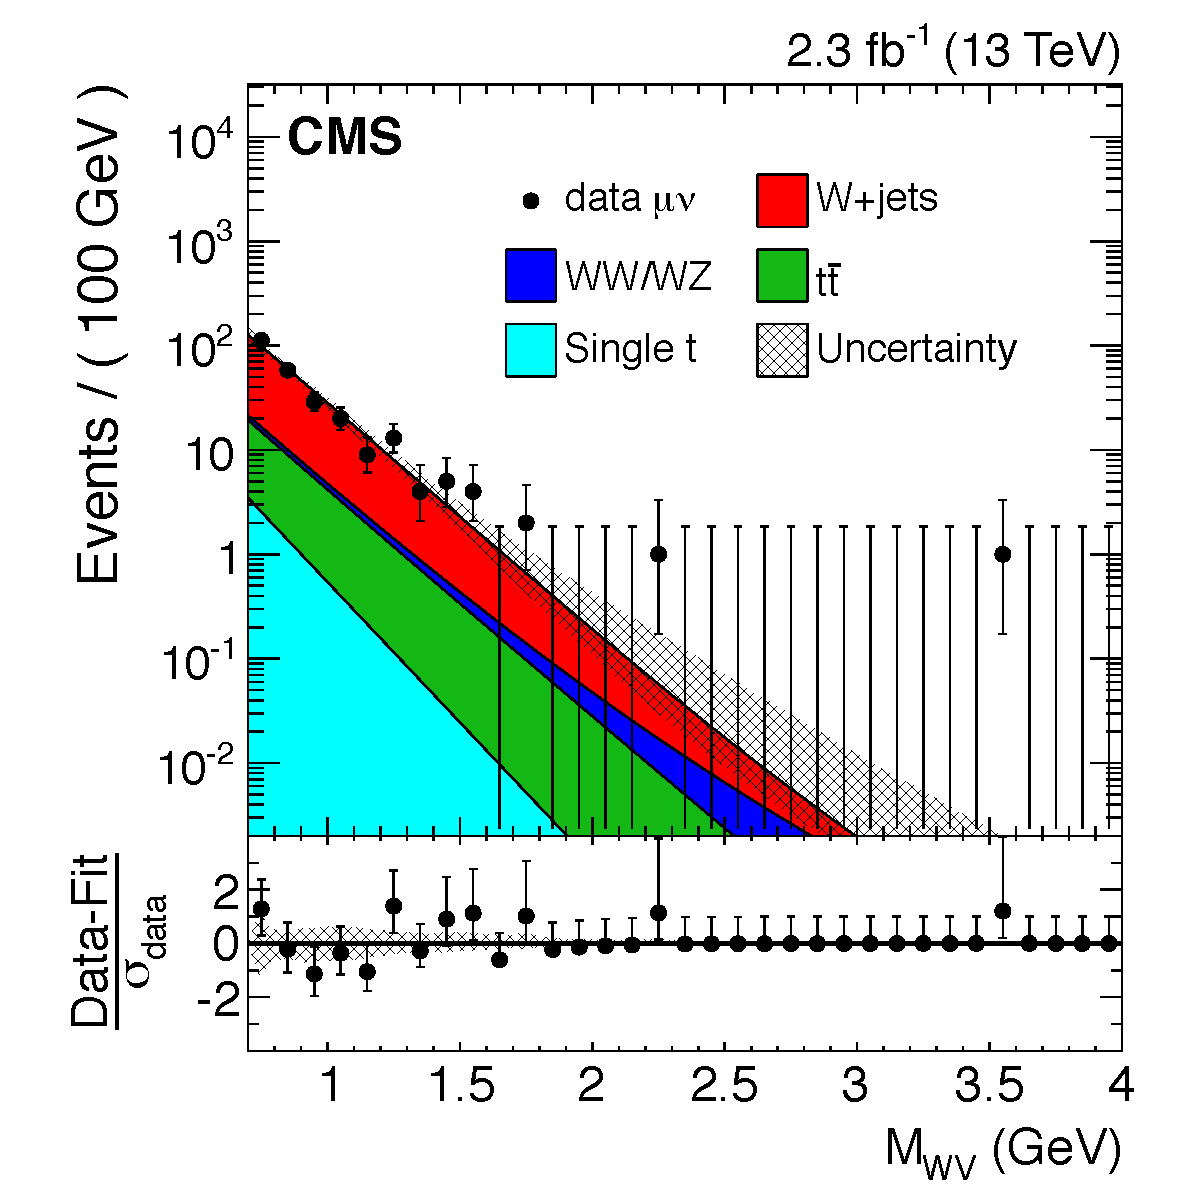
\includegraphics[width=0.5\textwidth]{\cheight/closureTest_HP_mu_regionB_mlvj.pdf}
\caption{Distributions in diboson invariant mass for data and the expected backgrounds for events inside the pruned mass region defined by $55 < \mJ < 65\GeV$ (B). The W+jets background distribution is extracted using events within $40 < \mJ < 55\GeV$ (A).}
\label{fig:mlvjSR_closureTest}
\end{figure}

%\FIXME{consider adding results with dijet function here or in the appendix}